% Stochastic Modeling and Simulation of Vehicle Headways on Highways
% Build: pdflatex main && bibtex main && pdflatex main && pdflatex main   (or upload this folder to Overleaf)
\documentclass[11pt,a4paper]{article}

\usepackage[T1]{fontenc}
\usepackage[utf8]{inputenc}
\usepackage{lmodern}
\usepackage[a4paper,margin=2.5cm]{geometry}
\usepackage{amsmath,amssymb}
\usepackage{graphicx}
\usepackage{booktabs,array,tabularx}
\usepackage{caption,subcaption}
\usepackage[section]{placeins}
\usepackage{enumitem}
\usepackage{listings}
\usepackage{xcolor}
\usepackage{tikz}
\usetikzlibrary{positioning,arrows.meta}
\usepackage{microtype}
\usepackage{xurl}
\setlength{\emergencystretch}{3em}
\usepackage[numbers,sort&compress]{natbib}
\usepackage[colorlinks=true,linkcolor=blue!50!black,citecolor=blue!50!black,urlcolor=blue!50!black]{hyperref}

\captionsetup{font=small,labelfont=bf}
\captionsetup[subfigure]{font=small}
\setlist{itemsep=2pt,topsep=3pt}
\setlength{\parskip}{3pt}
\renewcommand{\arraystretch}{1.12}
\newcolumntype{Y}{>{\raggedright\arraybackslash}X}
\lstset{language=Python,basicstyle=\ttfamily\scriptsize,breaklines=true,frame=single,numbers=left,
        numberstyle=\tiny\color{gray},keywordstyle=\bfseries,commentstyle=\itshape\color{gray},
        showstringspaces=false,xleftmargin=1.5em,captionpos=b,belowskip=1.2em}
\numberwithin{equation}{section}

\newcommand{\E}{\mathbb{E}}
\newcommand{\Var}{\operatorname{Var}}
\newcommand{\Prob}{\mathbb{P}}
\newcommand{\Wvec}{W_{\mathrm{vec}}}
\newcommand{\Wtime}{W_{\mathrm{time}}}
% Scalar results used in the text. Source: the run summarised in report.zip (lab PC, highD: all 60 recordings;
% NGSIM: I-80, recording period 1, MCMC 2 chains x 10,000 iterations, 5,000 warmup, seed 42). Table bodies are in tables/.
% Derived quantities (flow = 3600/mean headway, kappa = -ln b, recurrence = 1/pi) agree with the run's own printout.

% ---- samples ---------------------------------------------------------------------------------
\newcommand{\hdN}{1,225,460}
\newcommand{\ngN}{117,068}
\newcommand{\hdMean}{2.21}
\newcommand{\ngMean}{3.08}
\newcommand{\hdMedian}{1.66}
\newcommand{\ngMedian}{2.56}

% ---- proposed distribution (posterior means) ------------------------------------------------
\newcommand{\hdA}{0.954}
\newcommand{\hdB}{0.540}
\newcommand{\hdKappa}{0.617}
\newcommand{\ngA}{2.336}
\newcommand{\ngB}{0.524}
\newcommand{\ngKappa}{0.646}

% ---- goodness of fit -------------------------------------------------------------------------
\newcommand{\hdKLprop}{0.0036}
\newcommand{\ngKLprop}{0.0760}
\newcommand{\ngKLburr}{0.0016}
\newcommand{\hdKLmaxdiff}{0.0058}   % largest |ours - paper| over the seven distributions
\newcommand{\ngKLmaxdiff}{0.0311}
\newcommand{\hdWmaxdiff}{0.0006}
\newcommand{\ngWmaxdiff}{0.0110}    % gamma; 0.0003 or less for the other six

% ---- renewal process ---------------------------------------------------------------------------
\newcommand{\hdRate}{0.4520}
\newcommand{\ngRate}{0.3242}
\newcommand{\hdFlow}{1,627}
\newcommand{\ngFlow}{1,167}
\newcommand{\hdCV}{0.61}
\newcommand{\ngCV}{0.46}
\newcommand{\renewMeanMax}{0.4}     % percent, over t = 30, 60, 120, 300 s
\newcommand{\renewVarMax}{11.9}
\newcommand{\renewMeanShown}{0.2}   % percent, at the two horizons of Table~\ref{tab:renewal}
\newcommand{\renewVarShown}{3.8}

% ---- Markov regimes (stationary distribution = observed regime fractions) ---------------------
\newcommand{\hdPiC}{0.444}
\newcommand{\hdPiP}{0.431}
\newcommand{\hdPiF}{0.125}
\newcommand{\ngPiC}{0.094}
\newcommand{\ngPiP}{0.724}
\newcommand{\ngPiF}{0.182}

% ---- dependence of successive headways (highD, file order; see Section~\ref{sec:indep}) -------
\newcommand{\hdLagOne}{0.839}
\newcommand{\hdLagFive}{0.382}
\newcommand{\hdBand}{0.0018}

% ---- run time ----------------------------------------------------------------------------------
\newcommand{\hdMcmcTime}{1.8}
\newcommand{\ngMcmcTime}{1.7}

% ---- test suite: `uv run pytest -q tests` ----
\newcommand{\nTests}{46}


\title{\textbf{Stochastic Modeling and Simulation of Vehicle Headways on Highways:\\
A Bayesian Headway Distribution, Renewal Arrival Process, and Regime Markov Chain\\
Using highD and NGSIM Trajectory Datasets}}
\author{%
\begin{tabular}[t]{c}\textbf{Sanidhya Joshi}\\ (Team Leader)\\ Roll No.\ S20240010214\end{tabular}
\and
\begin{tabular}[t]{c}\textbf{Kaustabh Kadam}\\ \ \\ Roll No.\ S20240010114\end{tabular}
\and
\begin{tabular}[t]{c}\textbf{Dev Dharsandiya}\\ \ \\ Roll No.\ S20240010058\end{tabular}}
\date{International Institute of Information Technology, Sri City, India}

\begin{document}
\maketitle

%================================================================================================
\begin{abstract}
Headway, the time gap between successive vehicles in a lane, is a random quantity that governs highway capacity and
safety, yet no single standard distribution describes it across traffic conditions. This paper studies headway as a
stochastic system on two public trajectory datasets: highD (\hdN{} one-second headway samples from 60 German highway
recordings) and the I-80 data of NGSIM (\ngN{} samples from one recording period). A recently proposed two-parameter
density, $f(t\mid a,b)\propto b^{|t-a|}$, and six standard distributions are fitted by Metropolis--Hastings MCMC; vehicle
arrivals are modelled as a headway-driven renewal counting process; and car-following regimes are modelled as a
three-state Markov chain. By Kullback--Leibler divergence the proposed distribution is the best of the seven on highD
(\hdKLprop) and fourth on NGSIM (\ngKLprop), where the Burr distribution is best (\ngKLburr); the rankings match the published
study and the divergences agree with it to within \hdKLmaxdiff{} and \ngKLmaxdiff, respectively. Simulated renewal counts
agree with renewal theory (mean error at most \renewMeanMax\% and variance error at most \renewVarMax\% over four horizons),
and arrivals are markedly more regular than a Poisson stream (variance-to-mean ratios of \hdCV{} and \ngCV). The headway
sequence of a follower is strongly autocorrelated on highD (lag-1 coefficient about \hdLagOne), so the independence assumption of
the renewal model is only an approximation. The study also records two limitations of the estimation: the published likelihood does not condition on the
truncation of the sample to $[0.5,25]$~s, and one of the fourteen real-data posteriors (the shifted exponential on highD) did not converge.
\end{abstract}

\noindent\textbf{Keywords:} Traffic Headway; Stochastic Modelling; Bayesian Inference; Metropolis--Hastings Algorithm;
Renewal Process; Markov Chain; Traffic Flow; highD Dataset; NGSIM Dataset.

%================================================================================================
\section{Introduction}\label{sec:intro}

\subsection{Background and motivation}
The time headway between a vehicle and the vehicle ahead of it in the same lane is one of the basic microscopic
variables of traffic flow theory. The reciprocal of its mean is the flow that a lane can carry in car-following
conditions, short headways reduce the margin for braking, and its distribution is an input to capacity analysis, signal
timing and microscopic simulation~\cite{li2017survey,may1990}. Headways are random. They depend on driver behaviour,
vehicle type, speed, traffic volume and road geometry, so that no single deterministic value describes a lane, and the
shape of the distribution changes between free-flowing and congested traffic. A large literature has therefore proposed
and compared headway distributions without converging on a single model~\cite{li2017survey,leungbootnak}.

Leungbootnak et al.~\cite{leungbootnak} proposed a new two-parameter headway density, $f(t\mid a,b)\propto b^{|t-a|}$,
and compared it with six standard distributions on five trajectory datasets. This project reproduces that comparison on
two of the datasets, highD and NGSIM, and extends it in the direction of a course on applied stochastic modelling: the
fitted headway distribution is placed inside two stochastic processes (a renewal counting process for vehicle arrivals
and a Markov chain for car-following regimes), and each model is verified against theory, simulation and data.

\subsection{Research objectives}
\begin{enumerate}
  \item Estimate the parameters of seven headway distributions on highD and NGSIM by Bayesian MCMC and compare their
        goodness of fit.
  \item Reproduce the published goodness-of-fit results, and identify where and why they differ.
  \item Construct a renewal counting process from the headways, derive its theoretical moments, and compare them with
        simulated sample paths and with a Poisson process.
  \item Construct a three-state regime Markov chain, derive its stationary distribution and recurrence times, and
        state precisely what its estimation requires.
  \item Examine the assumptions behind the estimation (likelihood, sampler convergence, goodness-of-fit metrics) and
        the stochastic models (independence of headways, the Markov property).
\end{enumerate}

\subsection{Contributions}
The contributions are as follows.
(i)~A reproduction of the headway-distribution comparison of~\cite{leungbootnak} on highD and NGSIM, with an explicit
account of the sample and metric definitions needed to reproduce it.
(ii)~A renewal-process and a regime-Markov-chain model built on these headways, with their theory, simulation and
verification against each other.
(iii)~A statistical audit of the estimation. The likelihood of the published method does not condition on the truncation of the sample
to $[0.5,25]$~s (Section~\ref{sec:lik}); one real-data posterior, the shifted exponential on highD, did not converge
(Section~\ref{sec:conv}); and the Wasserstein distance and the KS test of the published study cannot be reproduced from its description
without further assumptions (Sections~\ref{sec:math} and~\ref{sec:gof}).
(iv)~A clear separation of what was verified mathematically, by simulation, and against real data (Section~\ref{sec:valid}).

\subsection{Organisation of the paper}
Section~\ref{sec:lit} reviews the literature. Section~\ref{sec:data} describes the datasets and preprocessing.
Section~\ref{sec:math} gives the mathematical background and Section~\ref{sec:framework} the proposed stochastic modelling
framework. Section~\ref{sec:method} describes the methodology, including the computational implementation.
Section~\ref{sec:results} presents the results, validation and discussion. Section~\ref{sec:limits} lists limitations and
future work, and Section~\ref{sec:conclusion} concludes. The appendix contains source code only.

%================================================================================================
\section{Literature Review}\label{sec:lit}

\subsection{Historical development of headway modelling}
Probabilistic descriptions of road traffic begin with Adams~\cite{adams1936}, who treated the arrival of vehicles at a
point as a random series and showed that, when arrivals are independent and uniformly likely in time, the number of
vehicles in an interval is Poisson distributed and the gaps between vehicles follow the negative exponential
distribution~\cite{adams1936,may1990}. The Poisson--exponential pair is attractive because it has one parameter and is
memoryless, but its density is largest at zero headway. Real drivers cannot follow at zero gap: vehicles have length, and
drivers need time to react. This inconsistency motivated modified forms. The literature reviewed in~\cite{leungbootnak}
and surveyed in~\cite{li2017survey} includes the shifted exponential, the hyper-exponential, the log-normal
distribution~\cite{greenberg1966}, the hyperlang distribution~\cite{dawson1968} and the semi-Poisson model of
Buckley~\cite{buckley1968}. Cowan~\cite{cowan1975} gave a structural argument: a headway is either a \emph{tracking}
headway, produced by a vehicle that is following its leader, or a \emph{free} headway, produced by a vehicle that is not,
and the four composite models M1--M4 mix these two components. A distinction that runs through the later literature is
between uninterrupted flow, where vehicles interact mainly with one another, and interrupted flow, where signals or stop
signs break the stream~\cite{hcm2000}; headways are generally shorter under the former~\cite{leungbootnak}.

\subsection{Classical distributions for headway}
Five families other than the exponential recur in the headway literature and in the comparison of this paper.
The \emph{log-normal} distribution is right-skewed with positive support and was applied to headways
early~\cite{greenberg1966}; with a location shift it excludes headways below a physical minimum. The \emph{Weibull}
distribution has a flexible hazard rate and contains the exponential as a special case~\cite{johnson1995}. The \emph{gamma} distribution
(an Erlang distribution when its shape is an integer) arises as the sum of independent exponential stages, which suggests
a car-following interpretation; the hyperlang of~\cite{dawson1968} is a related generalisation. The \emph{log-logistic}
distribution has a closed-form distribution function and a heavier tail than the log-normal. The three-parameter
\emph{Burr} distribution generalises the log-logistic family and spans a wide range of
shapes. Their advantages are simplicity and well-known properties; their common limitation is that
each describes a single regime, so that the best-fitting family changes with traffic conditions. Studies reviewed
in~\cite{leungbootnak} report log-normal fits for free-flowing traffic and log-logistic fits for congested traffic, and
Roy and Saha~\cite{roysaha2017} compare candidate models for two-lane roads under mixed traffic. Wang et
al.~\cite{wang2022} find that car-following-car and car-following-truck headways are described by log-logistic
distributions while truck-following headways are better described by gamma distributions, as reported
in~\cite{leungbootnak}. Composite and mixture models, such as the mixed distribution for urban roads of Li et
al.~\cite{li2021access}, fit more flexibly at the cost of more parameters and of a classification of traffic states.

\subsection{Heterogeneity and driver behaviour}
Headway depends on at least four factors. \emph{Vehicle type}: Hoogendoorn and Bovy~\cite{hoogendoorn1998} estimate
headway distributions per vehicle type, and Ye and Zhang~\cite{ye2009} analyse vehicle-type-specific headways from freeway
data. \emph{Speed}: Chen et al.~\cite{chen2010} show that headway and spacing distributions differ across speed ranges, and
Zou et al.~\cite{zou2014} construct a bivariate distribution for freeway speed and headway. \emph{Traffic condition and
density}: headway distributions have been fitted to expressway, two-lane and heterogeneous traffic~\cite{panichpapiboon2015,roysaha2017,maurya2016},
and as reviewed in~\cite{leungbootnak} the best-fitting family depends on the traffic condition. \emph{Driver behaviour}: Taieb-Maimon and Shinar~\cite{taieb2001}
study the minimum and the comfortable headways that drivers keep and how they relate to drivers' perception. Automated vehicles add a further
source of heterogeneity: Mahmassani~\cite{mahmassani2016} discusses the flow and operations considerations of mixed traffic of human-driven and automated
vehicles, and Wen et al.~\cite{wen2022} characterise the car-following behaviour of human drivers when following automated vehicles. Datasets from automated vehicles,
such as the Waymo open dataset~\cite{hu2022}, make driving-behaviour research of this kind possible, and~\cite{leungbootnak} includes two of them. The present study uses human-driven highway data only.

\subsection{Bayesian estimation in traffic modelling}
Bayesian inference treats the parameters $\theta$ of a distribution as random, with a prior $p(\theta)$ that encodes
what is known beforehand, and combines it with the likelihood of the data to give a posterior
$p(\theta\mid x)\propto p(x\mid\theta)p(\theta)$~\cite{gelman2013}. For distributions with several parameters this posterior
is rarely available in closed form and is explored by Markov chain Monte Carlo, in particular the Metropolis--Hastings
algorithm~\cite{metropolis1953,hastings1970}. A random-walk proposal is efficient when its scale is tuned: for
high-dimensional targets, the optimal acceptance rate is about 23\%~\cite{roberts1997}, and proposals can be adapted
during a warmup phase~\cite{haario2001}. Convergence is judged by running several chains and comparing between-chain with
within-chain variance~\cite{vehtari2021}. The advantages for headway modelling are that the posterior quantifies
parameter uncertainty, that priors regularise poorly identified parameters, and that all seven candidate distributions
are estimated in one framework. Wu et al.~\cite{wu2023} use Bayesian model averaging to combine
headway distributions, and Leungbootnak et al.~\cite{leungbootnak} estimate each distribution by Metropolis--Hastings, following their approach.

\subsection{Renewal processes in traffic flow}
A renewal process is a counting process whose inter-event times are independent and identically distributed~\cite{cox1962,ross1996}.
Taking the headways as inter-arrival times gives a model of the number of vehicles passing a point, with the Poisson
process as the special case of exponential headways. The renewal formulation is natural for traffic because its
distribution of inter-arrival times is free to be more regular than exponential: car following suppresses both very short
and very long gaps, so that counts in a fixed interval vary less than a Poisson process would predict. Whether real
headways are independent is a separate question, since a driver's gap to the leader changes gradually; the i.i.d.\ assumption
is therefore tested rather than assumed in this study (Section~\ref{sec:indep}).

\subsection{Markov chains in traffic regime modelling}
A finite Markov chain describes a system that moves between a small set of states with probabilities that depend only on
the current state~\cite{norris1997}. Chen et al.~\cite{chen2010} developed a Markov model for the headway and spacing
distribution of road traffic. Regime models of this kind need a definition of the states, an estimate of the transition
matrix from trajectories, and a check that the Markov property is adequate. Their useful outputs are the stationary
distribution, which gives the long-run share of time in each regime, and the mean recurrence time of each regime.

\subsection{Research gap and motivation}
The study being reproduced~\cite{leungbootnak} compares headway \emph{distributions} on five datasets. It does not place the
fitted distribution inside a stochastic process, does not examine whether successive headways of a vehicle are independent,
and does not report arrival-count behaviour or regime dynamics. It also leaves some details of its estimation and metrics
open (the treatment of truncation, the definition of the vectors in its Wasserstein distance, the NGSIM sample). Comparing
the proposed distribution with classical alternatives on highD and NGSIM, while adding a renewal and a Markov model and
verifying each of them, addresses these points and shows how far the published conclusions carry over to the structure
of real car-following data.

%================================================================================================
\section{Dataset Description and Preprocessing}\label{sec:data}

\subsection{The highD dataset}
highD~\cite{krajewski2018} contains trajectories of road users recorded by a drone above German highways. It comprises 60
recordings at 25~Hz. For each vehicle and frame, the tracking file gives the position, velocity, lane and the identifier
of the preceding vehicle in the same lane (\texttt{precedingId}, zero if there is none), together with the time headway to it
(\texttt{thw}); a metadata file gives the frame rate. highD describes uninterrupted highway flow of human-driven vehicles.

\subsection{The NGSIM dataset}
The Next Generation Simulation program of the U.S.\ Federal Highway Administration~\cite{ngsim} released vehicle
trajectories extracted from video of several roads. We use the I-80 data, recorded at 10~Hz. Each record gives the vehicle
identifier, frame, lane, the preceding vehicle (\texttt{Preceding}, zero if none) and the time headway
(\texttt{Time\_Headway}). The paper being reproduced~\cite{leungbootnak} used the reconstructed I-80 trajectories of
Montanino and Punzo~\cite{montanino2015}; the data used here is the original Data.gov export, which is not reconstructed.

\subsection{Sampling, filtering and headway extraction}
Following~\cite{leungbootnak}, headways are extracted as follows. (1)~One sample per second is kept for every following
vehicle (every 25th frame in highD, every 10th in NGSIM), so that the sampling rate is the same in both datasets.
(2)~Only records with a preceding vehicle in the same lane are kept. (3)~Headways below $\alpha=0.5$~s, which are generally
regarded as below the minimum safe headway, and above 25~s, which do not represent car following, are discarded. The
headway of a record is the dataset's own time-headway field: the time gap between a follower and its leader, not the
time between successive vehicles passing a fixed point. This distinction matters for the renewal model
(Section~\ref{sec:renewal}). The retained headways are ordered by vehicle and then time, and every stretch of consecutive
seconds of one vehicle is labelled as a \emph{trajectory run}. A new run starts whenever the vehicle changes or a second is
missing, which happens when the vehicle has no valid leader for a while. Runs are used to avoid counting transitions
between different vehicles (Section~\ref{sec:markovmethod}).

\subsection{Dataset selection rationale}
The two datasets differ in the way that matters for headway: highD records free-flowing highway traffic with short
headways, while the NGSIM sample has longer and more varied headways (Table~\ref{tab:data}). The NGSIM I-80 export contains two
recording periods, separated by gaps of more than ten minutes in the time stamp. The first period gives \ngN{}
headways with a mean of \ngMean~s; the second gives about 293\,000 headways with a mean of about 4.0~s. The paper does
not say which period it used. The fitted NGSIM parameters in its Table~3 imply mean headways between 2.8 and 3.1~s,
computed from the seven fitted distributions, which is close to the first period and far from the second. We therefore use
the first period; this is an inference from the published numbers, and not something the paper states.

\begin{table}[htbp]
\centering\small
\caption{Characteristics of the two datasets and of the headway samples used. Headways are in seconds; Std is the standard deviation.}
\label{tab:data}
\begin{tabularx}{\textwidth}{@{}lYY@{}}
\toprule
 & highD & NGSIM (I-80) \\
\midrule
Provider & RWTH Aachen University~\cite{krajewski2018} & U.S.\ Federal Highway Administration~\cite{ngsim} \\
Region and sensor & German highways; drone camera & I-80, California; fixed video cameras \\
Native frame rate & 25~Hz & 10~Hz \\
Flow regime & Uninterrupted, human-driven & Highway, human-driven \\
Selection used & all 60 recordings & first recording period \\
Leader and headway fields & \texttt{precedingId}, \texttt{thw} & \texttt{Preceding}, \texttt{Time\_Headway} \\
Sampling & one sample per second per follower & one sample per second per follower \\
Retained headways & \hdN & \ngN \\
Mean / median / Std (s) & \hdMean\ / \hdMedian\ / 1.73 & \ngMean\ / \ngMedian\ / 2.08 \\
\bottomrule
\end{tabularx}
\end{table}

%================================================================================================
\section{Mathematical Background}\label{sec:math}

\subsection{Probability distributions and truncation}
Seven distributions are compared (Table~\ref{tab:dists}): the proposed distribution of Section~\ref{sec:proposed} and
six standard ones, with the densities and the priors of~\cite{leungbootnak}. Headways are observed only in the window
$[\alpha,T]=[0.5,25]$~s. A distribution with density $f$ and distribution function $F$ \emph{conditioned on the window} has
density and distribution function
\begin{equation}\label{eq:trunc}
f_{\mathrm{w}}(t)=\frac{f(t)}{F(T)-F(\alpha)},\qquad
F_{\mathrm{w}}(t)=\frac{F(t)-F(\alpha)}{F(T)-F(\alpha)},\qquad \alpha\le t\le T .
\end{equation}
The fitted curves, the simulation of headways and every goodness-of-fit measure below use $F_{\mathrm w}$.

\begin{table}[htbp]
\centering\footnotesize
\caption{The seven distributions and the priors of~\cite{leungbootnak}. $\mathcal N(m,s)$ has mean $m$ and standard
deviation $s$; $\Gamma(k,r)$ has shape $k$ and rate $r$; $t_{\min}$ is the smallest observed headway.}
\label{tab:dists}
\begin{tabularx}{\textwidth}{@{}lYY@{}}
\toprule
Distribution & Density & Priors \\
\midrule
Proposed & $\dfrac{b^{|t-a|}}{Z(a,b)}$, $t\ge\alpha$ & $a\sim\mathcal N(0,10)$, $b\sim U(0,1)$ \\[1.5ex]
Shifted log-normal & $\dfrac{1}{(t-\gamma)\sigma\sqrt{2\pi}}\exp\!\Big\{-\dfrac{[\ln(t-\gamma)-\mu]^2}{2\sigma^2}\Big\}$, $t>\gamma$ &
 $\mu\sim\mathcal N(0,10)$, $\sigma\sim\Gamma(0.5,0.5)$, $\gamma\sim U(-10,t_{\min})$ \\[1.5ex]
Weibull & $\dfrac{\alpha t^{\alpha-1}}{\beta^{\alpha}}e^{-(t/\beta)^{\alpha}}$ & $\alpha,\beta\sim\Gamma(0.5,0.5)$ \\[1.5ex]
Log-logistic & $\dfrac{(\alpha/\beta)(t/\beta)^{\alpha-1}}{[1+(t/\beta)^{\alpha}]^{2}}$ & $\alpha,\beta\sim\Gamma(0.5,0.5)$ \\[1.5ex]
Gamma & $\dfrac{\beta^{\alpha}}{\Gamma(\alpha)}t^{\alpha-1}e^{-\beta t}$ & $\alpha,\beta\sim\Gamma(0.5,0.5)$ \\[1.5ex]
Burr & $\dfrac{\alpha\beta}{\lambda}(t/\lambda)^{\alpha-1}\big[1+(t/\lambda)^{\alpha}\big]^{-\beta-1}$ & $\alpha,\beta,\lambda\sim\Gamma(0.5,0.5)$ \\[1.5ex]
Shifted exponential & $\lambda e^{-\lambda(t-\gamma)}$, $t\ge\gamma$ & $\lambda\sim\Gamma(0.5,0.5)$, $\gamma\sim U(-10,t_{\min})$ \\
\bottomrule
\end{tabularx}
\end{table}

\subsection{Bayesian inference and the Metropolis--Hastings algorithm}
Let $\mathbf n=(n_1,\dots,n_{49})$ be the counts of headways in the 49 bins of width 0.5~s that tile $[0.5,25]$~s, and
$p_k(\theta)$ the model probability of bin $k$. The posterior is
\begin{equation}\label{eq:posterior}
\log p(\theta\mid\mathbf n)=\log p(\theta)+\sum_{k=1}^{49}n_k\log p_k(\theta)+\text{const.}
\end{equation}
The Metropolis--Hastings algorithm~\cite{metropolis1953,hastings1970} generates a Markov chain $\theta^{(0)},\theta^{(1)},\dots$ whose
stationary distribution is the posterior. From $\theta$ a candidate $\theta'=\theta+\varepsilon$ with $\varepsilon\sim\mathcal
N(0,s^2\Sigma)$ is proposed and accepted with probability
\begin{equation}\label{eq:accept}
\rho(\theta,\theta')=\min\Big\{1,\ \frac{p(\theta'\mid\mathbf n)}{p(\theta\mid\mathbf n)}\Big\},
\end{equation}
and otherwise the chain stays at $\theta$. The scale $s$ and covariance $\Sigma$ affect only the efficiency. For
random-walk proposals the optimal acceptance rate is near 23\%~\cite{roberts1997}.

\subsection{Convergence diagnostics}
For $C$ chains of $N$ draws, the split $\hat R$ of~\cite{vehtari2021} splits every chain in two, giving $m=2C$ sequences of
length $N/2$ with means $\bar\theta_j$, and compares the between-sequence variance $B$ with the within-sequence variance
$W$:
\begin{equation}\label{eq:rhat}
\hat R=\sqrt{\frac{\tfrac{n-1}{n}W+\tfrac1nB}{W}},\qquad n=\tfrac N2,\quad
B=\frac{n}{m-1}\sum_{j=1}^{m}(\bar\theta_j-\bar\theta)^2 .
\end{equation}
Values close to 1 indicate that the sequences agree; we flag $\hat R\ge1.05$. The effective sample size (ESS), obtained
from the autocorrelation of each chain, measures how many independent draws the chain is worth.

\subsection{Renewal processes and the Poisson process}
Let $H_1,H_2,\dots$ be i.i.d.\ positive random variables with mean $\mu$ and variance $\sigma^2$ and let $S_n=H_1+\dots+H_n$.
The counting process $N(t)=\max\{n: S_n\le t\}$ is a renewal process, with $\{N(t)\ge n\}=\{S_n\le t\}$. Its renewal function
$m(t)=\E N(t)$ satisfies $m(t)/t\to1/\mu$ (the elementary renewal theorem), and for a non-lattice distribution with finite
variance~\cite{cox1962,ross1996}
\begin{equation}\label{eq:renewal}
m(t)=\frac t\mu+\frac{\sigma^2-\mu^2}{2\mu^2}+o(1),\qquad \Var N(t)\sim\frac{\sigma^2t}{\mu^3},\qquad
N(t)\ \overset{\cdot}{\sim}\ \mathcal N\!\Big(\frac t\mu,\ \frac{\sigma^2t}{\mu^3}\Big).
\end{equation}
If $H$ is exponential then $N(t)$ is a Poisson process, with $\Var N(t)=\E N(t)=t/\mu$ for all $t$. In general
\begin{equation}\label{eq:dispersion}
\frac{\Var N(t)}{\E N(t)}\ \longrightarrow\ \frac{\sigma^2}{\mu^2}=:\mathrm{CV}^2,
\end{equation}
the squared coefficient of variation of the headway. A value below 1 means that arrivals are more regular than Poisson.

\subsection{Finite-state Markov chains}
A discrete-time Markov chain $(X_n)$ on a finite state space $S$ with transition matrix $P=(p_{ij})$ satisfies
$\Prob(X_{n+1}=j\mid X_n=i,X_{n-1},\dots)=p_{ij}$, and its $n$-step transition matrix is $P^{(n)}=P^n$ (the
Chapman--Kolmogorov equation)~\cite{norris1997}. If the chain is irreducible and aperiodic, $P^n\to\mathbf1\pi$, where the stationary
distribution is the solution of
\begin{equation}\label{eq:stationary}
\pi P=\pi,\qquad \sum_{i\in S}\pi_i=1 ,
\end{equation}
and the mean recurrence time of state $i$ is $1/\pi_i$. The maximum-likelihood estimate of $P$ from an observed path is
$\hat p_{ij}=n_{ij}/n_{i\cdot}$, where $n_{ij}$ is the number of observed transitions from $i$ to $j$.

\subsection{Goodness-of-fit metrics}
Four measures from~\cite{leungbootnak} are computed on the window-conditioned model.
The \emph{two-sample Kolmogorov--Smirnov} statistic $D=\sup_x|Q(x)-P(x)|$~\cite{massey1951} compares the empirical
distribution function $Q$ of the data with $P$ of a sample drawn from the fitted model.
The \emph{chi-square} statistic $\chi^2=\sum_i(O_i-E_i)^2/E_i$~\cite{pearson1900} is computed on the bin counts, with adjacent bins
merged until each merged bin has an observed count of at least 5.
The \emph{Kullback--Leibler divergence} of the observed bin probabilities $p_k$ from the model bin probabilities
$q_k$~\cite{kullback1951} is
\begin{equation}\label{eq:kl}
D_{KL}(P\|Q)=\sum_k p_k\log\frac{p_k}{q_k}.
\end{equation}
The \emph{Wasserstein distance} of order~1 between two samples of equal size is the mean absolute difference of their order statistics,
$\frac1n\sum_{i=1}^n|X_{(i)}-Y_{(i)}|$~\cite{vallender1974}; this is Eq.~17 of~\cite{leungbootnak} with $p=1$. Its definition is ambiguous
because the paper does not say what $X$ and $Y$ are. We evaluate it in two ways that must not be confused:
\begin{align}
\Wvec&=\frac1{49}\sum_{i=1}^{49}\big|p_{(i)}-q_{(i)}\big|, &&\text{(sorted bin-probability vectors, unitless)}\label{eq:wvec}\\
\Wtime&=\int\big|F_{\mathrm{obs}}(t)-F_{\mathrm w}(t)\big|\,dt, &&\text{(headway distributions on the time axis, seconds)}\label{eq:wtime}
\end{align}
where $p_{(i)}$ and $q_{(i)}$ are the observed and model bin probabilities in increasing order. $\Wvec$ treats the 49 probabilities as two samples and
is blind to \emph{where} on the time axis each bin lies. $\Wtime$ is the conventional one-dimensional Wasserstein distance
between the two headway distributions, evaluated on the 49 bin centres. The values printed in~\cite{leungbootnak}
(of order $10^{-3}$) are only compatible with $\Wvec$, so that is the quantity compared with the paper; $\Wtime$ is reported
alongside it because it is the conventional distance.

%================================================================================================
\section{Proposed Stochastic Modelling Framework}\label{sec:framework}

\subsection{Terminology}
Five terms are kept apart throughout (Table~\ref{tab:terms}). The distinction between a \emph{time headway} and a
\emph{detector inter-arrival time} is central: the first is measured between two vehicles at one instant, the second between
two vehicles passing one place.

\begin{table}[htbp]
\centering\small
\caption{Terminology used in this paper.}\label{tab:terms}
\begin{tabularx}{\textwidth}{@{}lY@{}}
\toprule
Term & Meaning here \\
\midrule
Time headway $H$ & Time gap between a following vehicle and its leader in the same lane at one instant, as reported by the datasets
 (\texttt{thw}, \texttt{Time\_Headway}). \\
Detector inter-arrival time & Time between two successive vehicles of a lane crossing a fixed cross-section. Not used directly; see Section~\ref{sec:renewal}. \\
Renewal inter-arrival distribution & The distribution assigned to the i.i.d.\ gaps of the renewal process $N(t)$; here, the time-headway distribution. \\
Vehicle trajectory & The sequence of positions of one vehicle over time; a \emph{run} is a stretch of consecutive seconds of it that enters the sample. \\
Traffic regime & One of three classes of time headway of a follower (close following, stable platoon, free flow), Section~\ref{sec:markov}. \\
\bottomrule
\end{tabularx}
\end{table}

\subsection{Bayesian headway distribution model}\label{sec:proposed}
The proposed density is
\begin{equation}\label{eq:density}
f(t\mid a,b)=\frac{b^{\,|t-a|}}{Z(a,b)},\qquad t\ge\alpha=0.5\text{ s},\quad 0<b<1 .
\end{equation}
With $\kappa=-\ln b>0$ it is $f\propto e^{-\kappa|t-a|}$, a Laplace (double-exponential) density centred at $a$ and truncated to
$t\ge\alpha$. For $a\ge\alpha$ the density has its mode at $a$, and integrating separately on $[\alpha,a]$ and $[a,\infty)$ gives the
normalising constant $Z=(2-b^{a-\alpha})/\kappa$ and the distribution function
\begin{equation}\label{eq:cdf}
F(t)=\begin{cases}
\dfrac{b^{a-t}-b^{a-\alpha}}{2-b^{a-\alpha}}, & \alpha\le t\le a,\\[2ex]
\dfrac{2-b^{a-\alpha}-b^{t-a}}{2-b^{a-\alpha}}, & t\ge a .
\end{cases}
\end{equation}
For $a<\alpha$ the density decreases on $[\alpha,\infty)$, with $Z=b^{\alpha-a}/\kappa$ and $F(t)=1-b^{t-\alpha}$. Equation~\eqref{eq:cdf} agrees with the
closed form of~\cite{leungbootnak} and is checked against numerical integration in the test suite
(Section~\ref{sec:valid}). It gives an inverse-transform sampler: with $c=b^{a-\alpha}$ and $u\sim U(0,1)$,
\begin{equation}\label{eq:sampler}
t=\begin{cases}
a-\ln\!\big(u(2-c)+c\big)/\ln b, & u\le F(a),\\[0.5ex]
a+\ln\!\big((1-u)(2-c)\big)/\ln b, & u>F(a).
\end{cases}
\end{equation}
The parameters have a direct reading: $a$ is the most frequent headway (the mode), and $\kappa$ is the exponential rate at which the density
falls on both sides of it. Because the decay rate is the same on both sides of $a$, the density is symmetric about its mode apart from the truncation at $\alpha$,
which constrains what shapes it can take (Section~\ref{sec:disc}).

\subsection{Renewal arrival process}\label{sec:renewal}
\paragraph{Definition.} The headways $H_1,H_2,\dots$ of a lane are modelled as i.i.d.\ draws from a headway distribution
(the data or a fitted distribution), and the number of vehicles that have passed a point by time $t\ge0$ is the renewal
counting process $N(t)$ of Section~\ref{sec:math}, with state space $\{0,1,2,\dots\}$ and continuous time. The theory of
Eqs.~\eqref{eq:renewal}--\eqref{eq:dispersion} then gives the expected number of arrivals, its variance and its
distribution.

\paragraph{What this model assumes.} The model is \emph{headway-driven}: it uses the time headway between a follower and its leader
as the inter-arrival time. The two coincide when vehicles keep a constant speed between the leader's and the follower's
passage of a point, but not in general, and the datasets report $H$ at one instant, not detector crossing times. Detector crossing
times could be reconstructed from the trajectories (the position and the time at which each vehicle crosses a fixed
cross-section), but this was not done; the renewal process should be read as a model of arrivals that is
consistent with the observed headway distribution, not as a measured arrival process. The second assumption is that the
headways are independent, which is tested in Section~\ref{sec:indep}.

\subsection{Markov chain for traffic regimes}\label{sec:markov}
\paragraph{State space and time.} Each retained one-second sample of a follower is assigned a regime
\begin{equation}\label{eq:regimes}
X_n=\begin{cases}
\text{close following} & 0.5\le h<1.5\ \text{s},\\
\text{stable platoon} & 1.5\le h<4\ \text{s},\\
\text{free flow} & 4\le h\le25\ \text{s},
\end{cases}
\end{equation}
where $n$ indexes consecutive seconds of one vehicle's trajectory. The sequence $(X_n)$ is modelled as a time-homogeneous,
first-order Markov chain on $S=\{\text{close, platoon, free}\}$ with discrete time. The thresholds are modelling
choices, not estimated quantities.

\paragraph{Estimation and quantities.} $P$ is estimated by transition counts, $\hat p_{ij}=n_{ij}/n_{i\cdot}$, where only
pairs of consecutive samples in the \emph{same trajectory run} are counted (Section~\ref{sec:markovmethod}). The chain gives the
stationary distribution~\eqref{eq:stationary}, the mean recurrence times $1/\pi_i$ and the transient distribution
$\pi(n)=\pi(0)P^n$. A mean recurrence time is the expected number of seconds between successive visits of a trajectory to the
regime, assuming that the chain is stationary.

%================================================================================================
\section{Methodology}\label{sec:method}

\subsection{Overall research workflow}
The workflow has four stages (Figure~\ref{fig:workflow}): data are loaded and reduced to one-second headways;
seven distributions are fitted by MCMC and evaluated; the renewal process and the Markov chain are built from the
headways; and each stage is verified (Section~\ref{sec:valid}). All stages are run by one script and write
their tables and figures to disk.

\begin{figure}[htbp]
\centering
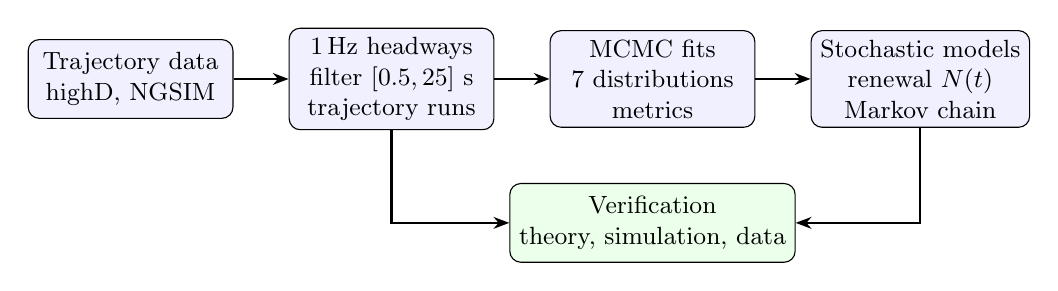
\begin{tikzpicture}[node distance=7mm, every node/.style={font=\small},
  box/.style={draw,rounded corners,align=center,minimum height=10mm,minimum width=26mm,fill=blue!6},
  arr/.style={-{Stealth[length=2mm]},thick}]
  \node[box] (d) {Trajectory data\\ highD, NGSIM};
  \node[box,right=of d] (h) {1\,Hz headways\\ filter $[0.5,25]$ s\\ trajectory runs};
  \node[box,right=of h] (m) {MCMC fits\\ 7 distributions\\ metrics};
  \node[box,right=of m] (s) {Stochastic models\\ renewal $N(t)$\\ Markov chain};
  \node[box,below=of m,fill=green!8] (v) {Verification\\ theory, simulation, data};
  \draw[arr] (d)--(h); \draw[arr] (h)--(m); \draw[arr] (m)--(s); \draw[arr] (h) |- (v); \draw[arr] (s) |- (v);
\end{tikzpicture}
\caption{Workflow of the study.}\label{fig:workflow}
\end{figure}

\subsection{Data acquisition and preprocessing}
The loaders read each recording or the NGSIM CSV and apply the extraction of Section~\ref{sec:data}: one-second
sampling, requirement of a preceding vehicle, and the window $[0.5,25]$~s. NGSIM records are selected by location (I-80) and
by recording period, and are sorted by vehicle and time, because the raw export is not in that order. The loaders can also return the
trajectory-run label of every headway. The highD recordings are processed in parallel, one worker per recording.

\subsection{Headway distribution selection}
The candidate set is the seven distributions of Table~\ref{tab:dists}, fixed in advance by the study being reproduced.
Selection is by the goodness-of-fit measures of Section~\ref{sec:math}, and no model is chosen by a test of significance, since all
of them are rejected on samples of this size (Section~\ref{sec:gof}).

\subsection{Bayesian parameter estimation}\label{sec:bayes}
Each distribution is fitted separately to each dataset, using the log-posterior of Eq.~\eqref{eq:posterior} with the priors of
Table~\ref{tab:dists} and the 49 bin counts. This binned likelihood costs the same per step whatever the sample size and is exact up to the
0.5~s bin resolution. Two likelihoods are implemented. The \emph{paper} likelihood uses each distribution's own density, so
that $\sum_kp_k(\theta)<1$ because mass outside $[0.5,25]$~s is lost; this is the method of~\cite{leungbootnak} and is the one used for all
real-data results reported here. The \emph{truncated} likelihood uses the conditioned probabilities of Eq.~\eqref{eq:trunc}, which sum to
one and are the exact likelihood for a sample truncated to the window; it is selectable in the code (Section~\ref{sec:lik}), but was not used for the real-data results.

\subsection{Metropolis--Hastings sampling procedure}
Two chains of 10\,000 iterations are run for each fit, the first 5\,000 being warmup, as in~\cite{leungbootnak}. The procedure is:
\begin{enumerate}
  \item \textbf{Initialise.} Chain~1 starts at the maximum a posteriori (MAP) point found by the Nelder--Mead simplex; chain~2 starts from this point
        scaled by 1.05 if that point is feasible, and from the MAP point otherwise.
  \item \textbf{Propose.} $\theta'=\theta+s\,L\,z$ with $z\sim\mathcal N(0,I)$ and $LL^{\top}=\Sigma$; initially
        $\Sigma=\operatorname{diag}\{(0.1\max(|\theta_i|,0.5))^2\}$ and $s=2.38/\sqrt d$ for $d$ parameters.
  \item \textbf{Accept or reject} with the probability of Eq.~\eqref{eq:accept}.
  \item \textbf{Adapt during warmup only.} Every 100 iterations $s$ is multiplied by $\operatorname{clip}\{\exp[0.8(r-0.234)],0.5,2\}$, where $r$ is the recent acceptance
        rate, and every 500 iterations $\Sigma$ is re-estimated from the last 1\,000 draws. Nothing is adapted after warmup, which preserves the stationary distribution.
  \item \textbf{Estimate.} The point estimate is the mean of the 10\,000 retained draws (2 chains of 5\,000).
\end{enumerate}
The code samples the shifted exponential's threshold $\gamma<t_{\min}$ through $v=\log(t_{\min}-\gamma)$, with the Jacobian $e^{v}$ added to the log-density, which is the exact change
of variables for the uniform prior on $\gamma$ (Section~\ref{sec:conv}). This was added after the real-data runs reported here and has not been applied to them.

\subsection{Goodness-of-fit evaluation}\label{sec:gofmethod}
For each fit, the window-conditioned model is evaluated with the four measures of Section~\ref{sec:math}: the two-sample KS statistic of
the data against a sample of $\min(n,50\,000)$ draws from the fitted model, the chi-square statistic on the merged bins, $D_{KL}$ of Eq.~\eqref{eq:kl},
and $\Wvec$ and $\Wtime$ of Eqs.~\eqref{eq:wvec}--\eqref{eq:wtime}.

\subsection{Renewal process construction}
For each dataset the renewal process is built on the empirical headways of the sample. The mean $\mu$ and variance $\sigma^2$ of the headway give $m(t)$,
$\Var N(t)$ and the dispersion $\sigma^2/\mu^2$ of Eqs.~\eqref{eq:renewal}--\eqref{eq:dispersion}, and the lane flow $3600/\mu$ vehicles per hour.

\subsection{Markov chain construction}\label{sec:markovmethod}
Headways are mapped to regimes by Eq.~\eqref{eq:regimes}. The transition matrix is estimated from \emph{within-run} pairs only: the pair
$(x_i,x_{i+k})$ is used only if both samples carry the same trajectory-run label. Since a run is a stretch of consecutive seconds of one vehicle, this
excludes every transition between two vehicles and every transition across a gap in time. For $k>1$ the same rule gives the empirical $k$-step transition
frequencies used in the Chapman--Kolmogorov check. The stationary distribution is obtained by solving Eq.~\eqref{eq:stationary}
by least squares.

\subsection{Simulation design}
\paragraph{Renewal paths.} For $M=2\,000$ paths, headways are drawn independently with replacement from the sample and cumulated to arrival times $S_n$; $N(t)$ is
the number of arrivals up to $t$, at the horizons $t=30,60,120,300$~s. Five paths are plotted. For the Markov chain, sample paths are generated from
the estimated $P$. All random numbers come from seeded generators (seed 42).
\paragraph{Fitted-model sampling.} Headways from a fitted distribution are drawn by inverting the window-conditioned distribution function on a
grid of 50\,001 points, for all seven distributions. For the proposed distribution Eq.~\eqref{eq:sampler} is the exact inverse of the unconditioned distribution function.

\subsection{Statistical validation strategy}\label{sec:valstrat}
Three kinds of validation are kept distinct, because agreement of a simulation with its own theory does not validate the model.
\begin{enumerate}
  \item \textbf{Mathematical verification}: the closed forms are correct. Automated tests check the distribution function against numerical integration, that every density integrates to one,
        and that the derivative of each distribution function is its density.
  \item \textbf{Simulation verification}: the code does what the mathematics says. Automated tests check that the sampler recovers the known parameters of a distribution from a sample drawn from it, and the simulated renewal moments are
        compared with Eq.~\eqref{eq:renewal}.
  \item \textbf{Empirical validation}: the model describes the real data. The fitted distributions are compared with the observed histograms by the four metrics; the assumptions of
        the renewal and Markov models are tested on the real sequences (autocorrelation, Chapman--Kolmogorov, first- against second-order); and the results are compared with the published ones.
\end{enumerate}

\subsection{Computational implementation}\label{sec:impl}
The implementation is a Python package, \texttt{headway/}, with a driver script, \texttt{run.py}. It uses NumPy, SciPy, pandas and Matplotlib; the
Metropolis--Hastings sampler is written from scratch because the PyMC3/Theano combination of the original study is not available for recent Python versions.
The modules are organised by role:
\begin{itemize}
  \item \texttt{distributions.py}: the seven densities and distribution functions, the priors, and the conditioned quantities of Eq.~\eqref{eq:trunc};
  \item \texttt{mcmc.py} and \texttt{fit.py}: the sampler, the binned posterior with both likelihoods, the MAP start, and the threshold reparametrisation;
  \item \texttt{metrics.py} and \texttt{diagnostics.py}: the goodness-of-fit measures, split $\hat R$ and the effective sample size;
  \item \texttt{datasets/}: the highD and NGSIM loaders and the trajectory-run labelling;
  \item \texttt{stochastic\_process.py}, \texttt{simulation.py} and \texttt{validation.py}: the renewal process and Markov chain, headway simulation, and the quantitative checks;
  \item \texttt{plots.py}: all figures.
\end{itemize}
Independent chains and independent recordings are run in parallel on all CPU cores with a shared process pool; every random generator is seeded, so that results are reproducible.
Running \texttt{run.py} fits all seven distributions to both datasets, evaluates them, runs the stochastic analyses and writes the tables (CSV) and figures that this paper uses;
the full benchmark of this study took \hdMcmcTime~s of MCMC on highD and \ngMcmcTime~s on NGSIM. The automated test suite (\nTests{} tests) covers the distributions, sampler,
loaders, metrics and stochastic processes. The code that matters for the method is reproduced in the appendix, extracted directly from the repository.

%================================================================================================
\section{Results and Discussion}\label{sec:results}

\subsection{Simulation results}\label{sec:sim}
\subsubsection{Renewal arrival process}
Figure~\ref{fig:paths} shows five simulated sample paths of the arrival count $N(t)$ for each dataset, with the renewal function $m(t)$ of
Eq.~\eqref{eq:renewal}. The paths scatter around $m(t)$; on highD the five paths span roughly 128 to 147 vehicles at $t=300$~s, against $m(300)=135.4$ (read from the figure). Table~\ref{tab:renewal} compares 2\,000 simulated paths with renewal theory. The
simulated means agree with $m(t)$ to within \renewMeanShown\% at the two horizons shown, and the simulated variances to within \renewVarShown\%. Over all four horizons
simulated (30, 60, 120 and 300~s) the largest errors are \renewMeanMax\% in the mean and \renewVarMax\% in the variance; the largest variance error
occurs at one of the two horizons not tabulated, and a variance estimated from 2\,000 paths has a Monte Carlo error of about 3\%.
This is a verification that the simulation implements Eq.~\eqref{eq:renewal}, not a validation of the model against data.

\begin{figure}[htbp]
\centering
\begin{subfigure}{0.49\textwidth}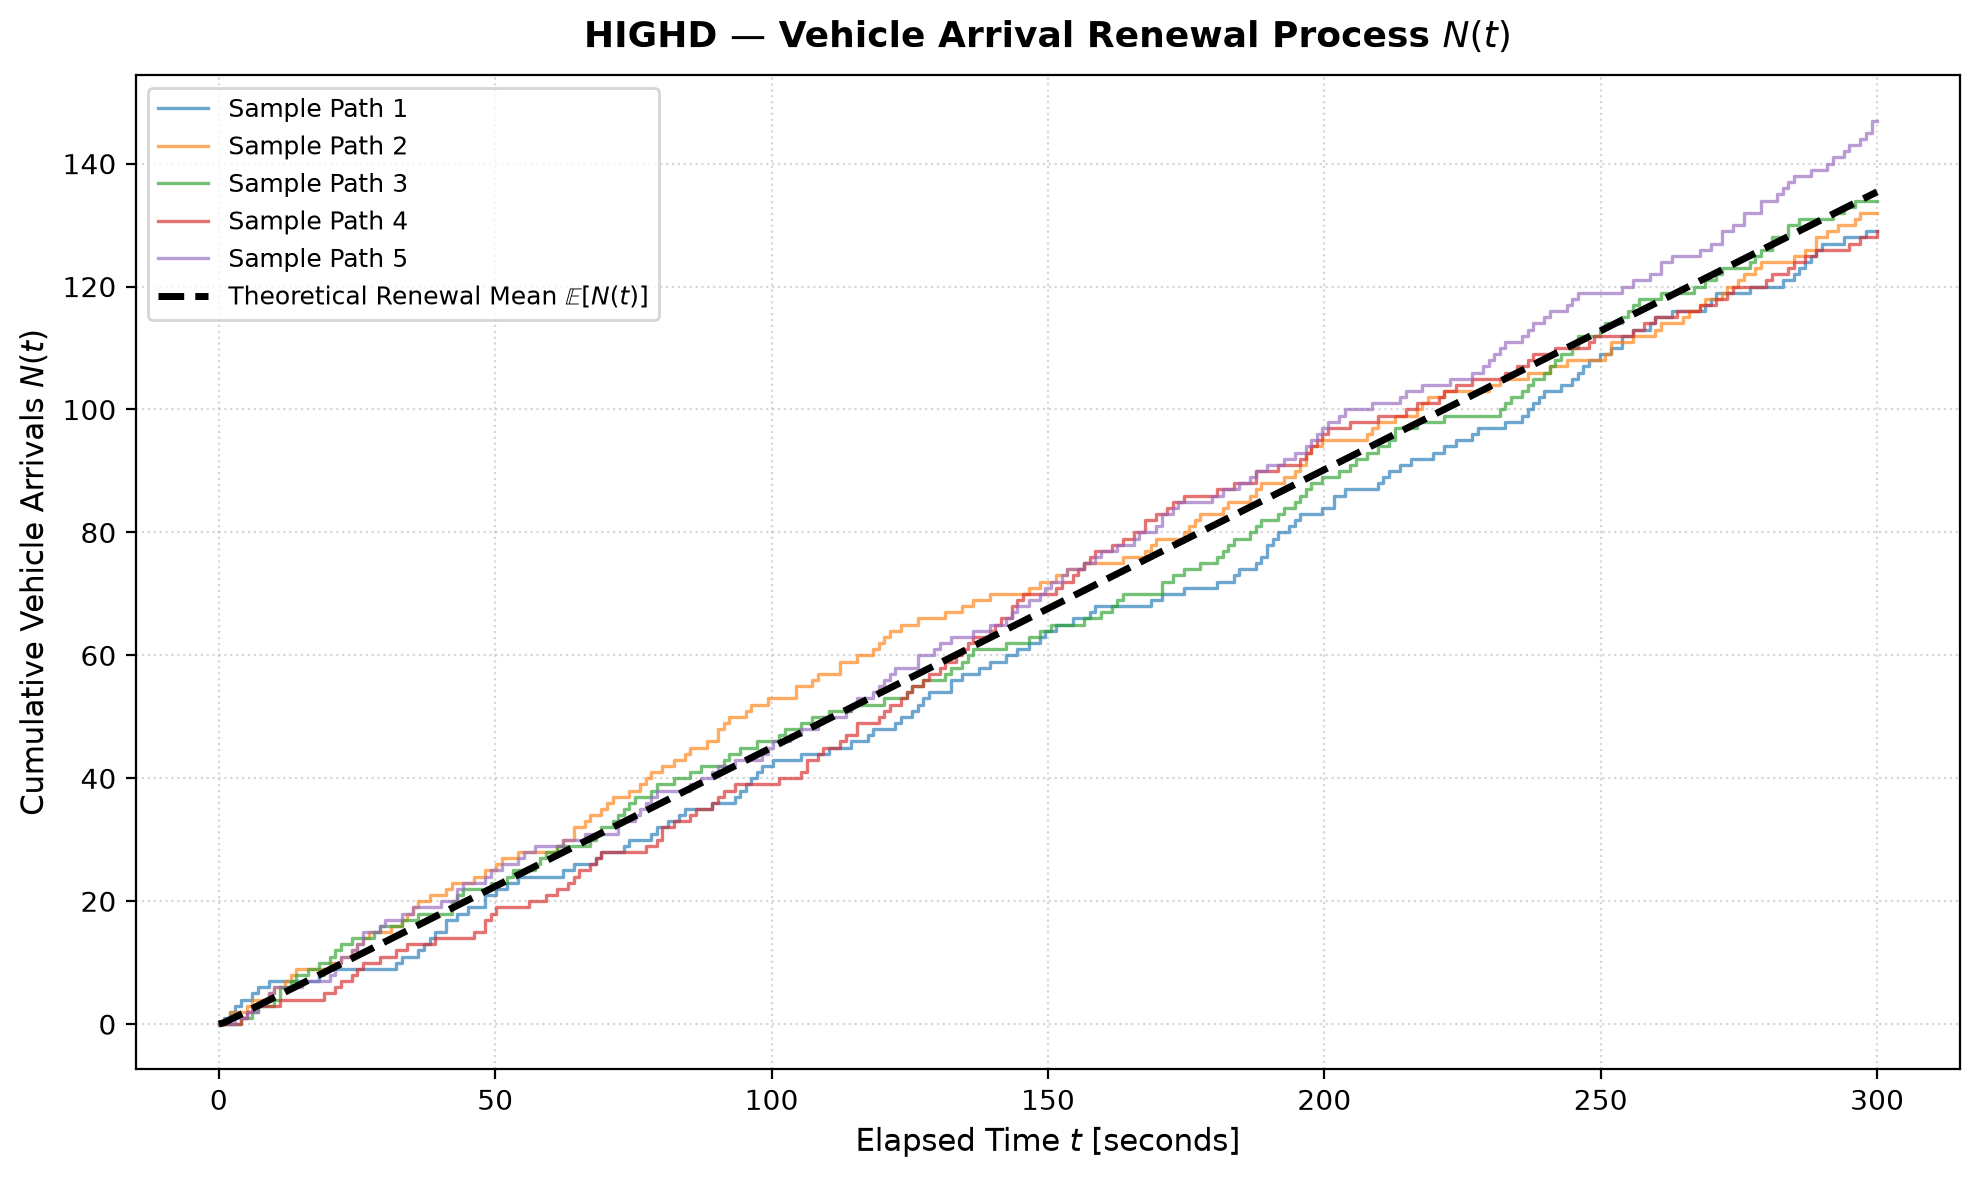
\includegraphics[width=\linewidth]{figures/highd_sample_paths.png}\caption{highD}\end{subfigure}\hfill
\begin{subfigure}{0.49\textwidth}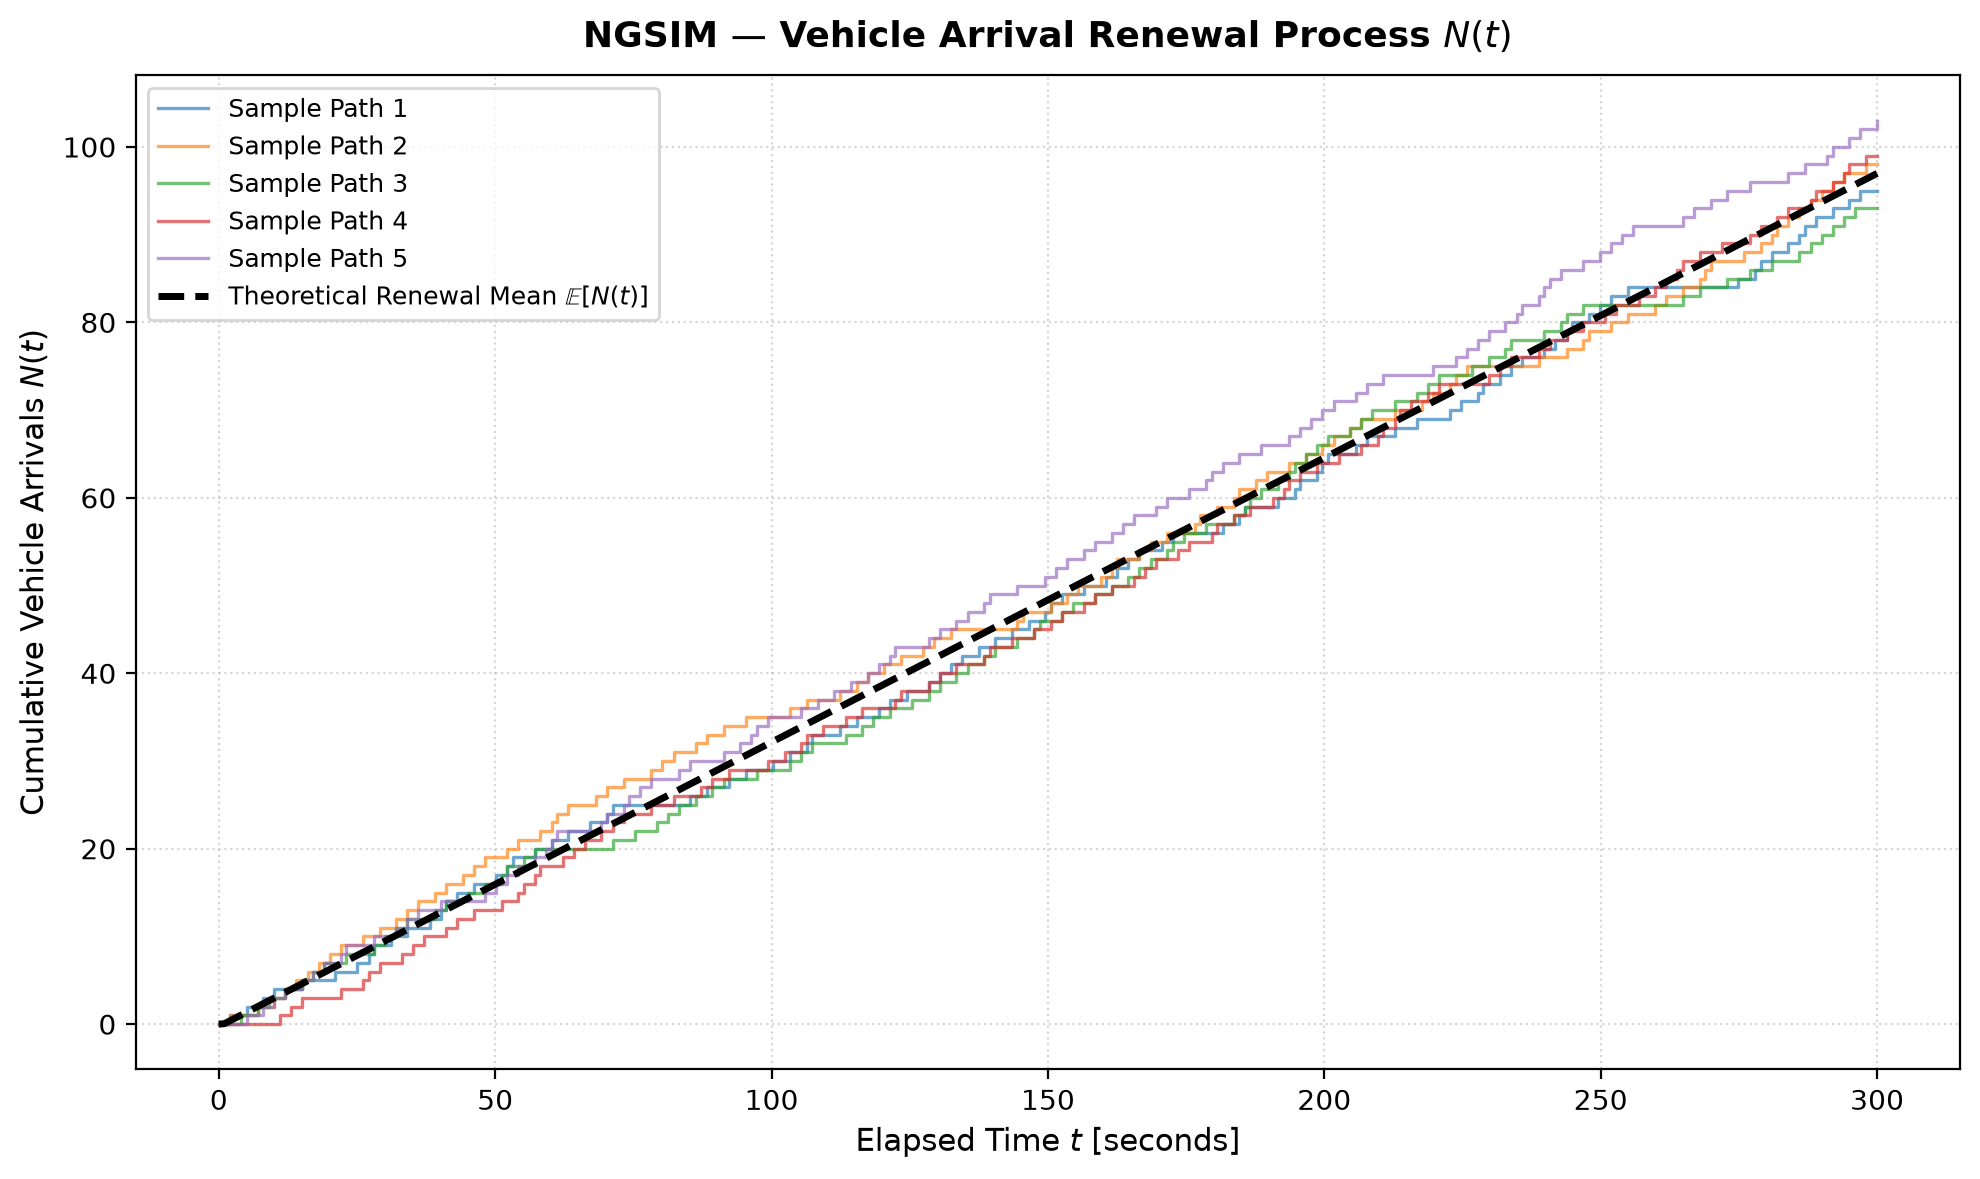
\includegraphics[width=\linewidth]{figures/ngsim_sample_paths.png}\caption{NGSIM}\end{subfigure}
\caption{Five simulated sample paths of the vehicle arrival count $N(t)$ and the theoretical renewal function $m(t)$ (dashed).}\label{fig:paths}
\end{figure}

\begin{table}[htbp]
\centering\footnotesize
\caption{Simulated renewal counts (2\,000 paths) against renewal theory, Eq.~\eqref{eq:renewal}. ``Var if Poisson'' is the variance of a Poisson process of the same rate; errors are relative to theory.}
\label{tab:renewal}
\begin{tabular}{@{}lrrrrrrrr@{}}
\toprule
Dataset & $t$ (s) & $\E N$ sim & $\E N$ theory & $\Var N$ sim & $\Var N$ theory & $\Var$ if Poisson & mean err & var err \\
\midrule
highD & 60 & 26.86 & 26.93 & 16.86 & 16.56 & 27.12 & 0.23\% & 1.8\% \\
NGSIM & 60 & 19.15 & 19.18 & 8.54 & 8.86 & 19.45 & 0.16\% & 3.6\% \\
highD & 300 & 135.57 & 135.41 & 85.94 & 82.81 & 135.60 & 0.12\% & 3.8\% \\
NGSIM & 300 & 96.99 & 96.98 & 44.85 & 44.28 & 97.26 & 0.00\% & 1.3\%
\\
\bottomrule
\end{tabular}
\end{table}

The variance of the count is far below that of a Poisson process: at $t=300$~s it is 85.9 on highD against 135.6 for a Poisson process of the same rate, and 44.9 on NGSIM
against 97.3. The variance-to-mean ratio of Eq.~\eqref{eq:dispersion} is \hdCV{} on highD and \ngCV{} on NGSIM, where a Poisson process has 1. Figure~\ref{fig:counts} shows the whole distribution
of $N(60)$. At $t=60$~s the largest gap between the simulated count distribution and the renewal-theory normal approximation is 0.022 on highD and 0.029 on NGSIM, while the gap to a Poisson distribution
is 0.071 and 0.126; the normal approximation of Eq.~\eqref{eq:renewal} describes the simulated counts much better than the Poisson distribution does. The renewal rates are \hdRate{} veh/s on highD and \ngRate{}
veh/s on NGSIM, i.e.\ \hdFlow{} and \ngFlow{} veh/h/lane. These are the reciprocals of the mean headways of followers who have a leader, so they describe car-following states and are not measured detector flows.

\begin{figure}[htbp]
\centering
\begin{subfigure}{0.49\textwidth}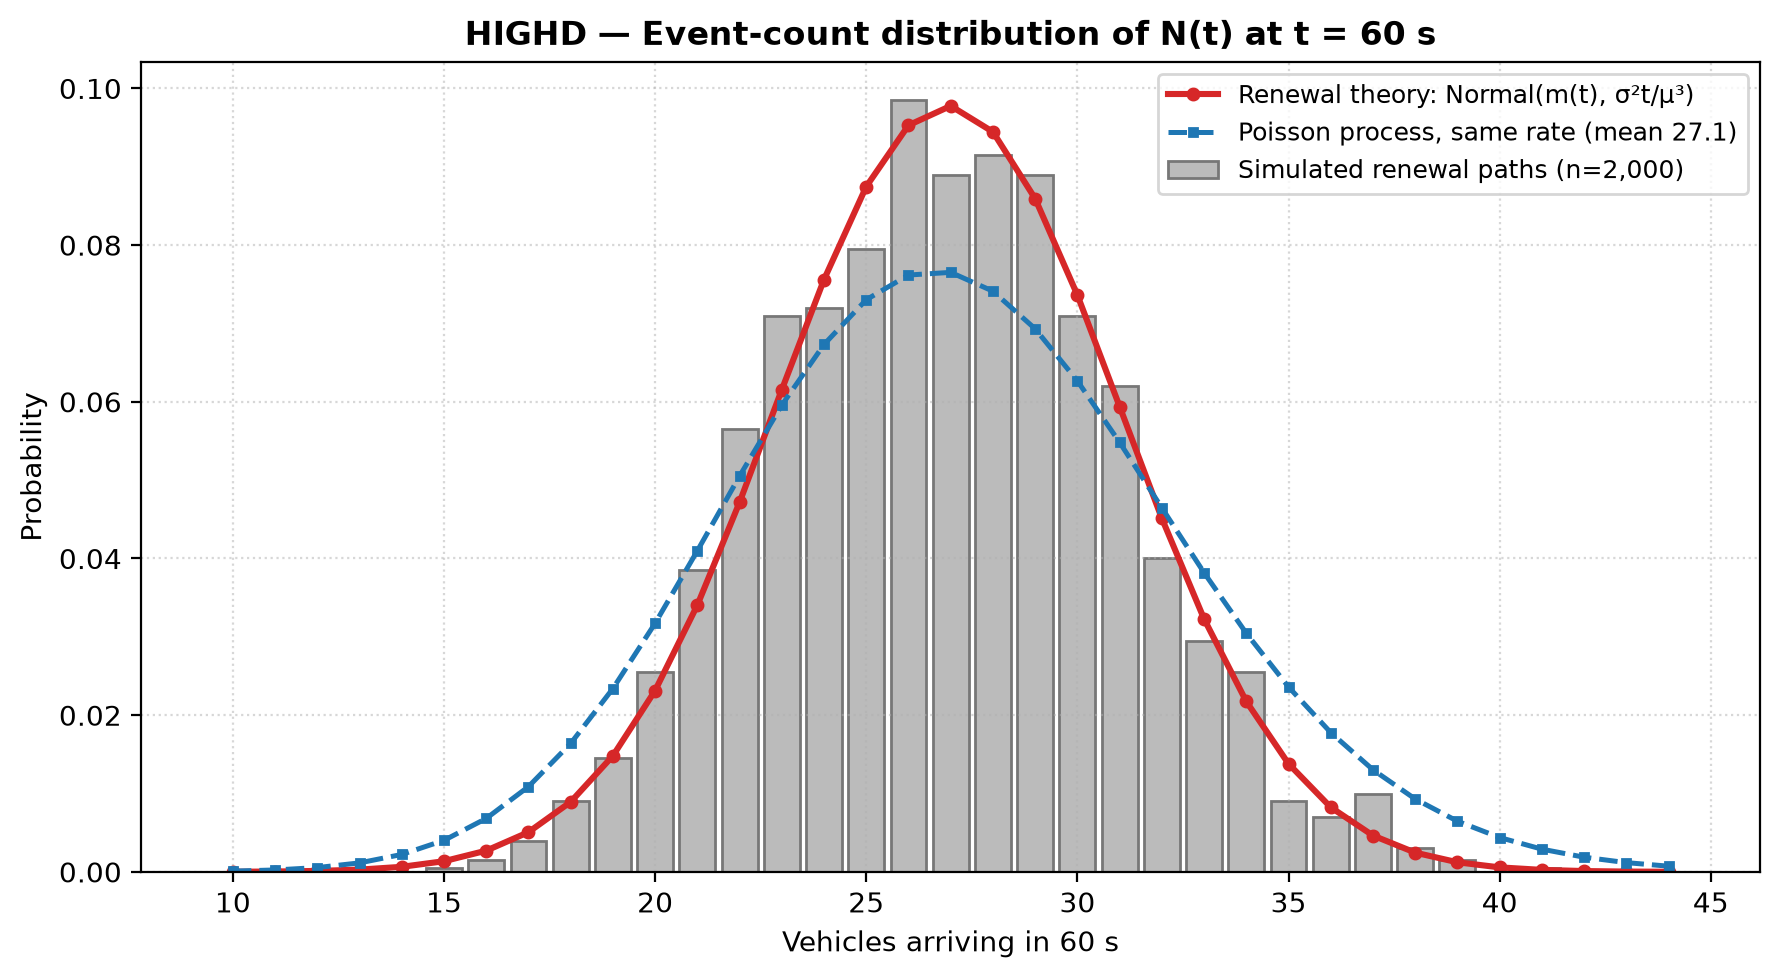
\includegraphics[width=\linewidth]{figures/highd_event_count.png}\caption{highD}\end{subfigure}\hfill
\begin{subfigure}{0.49\textwidth}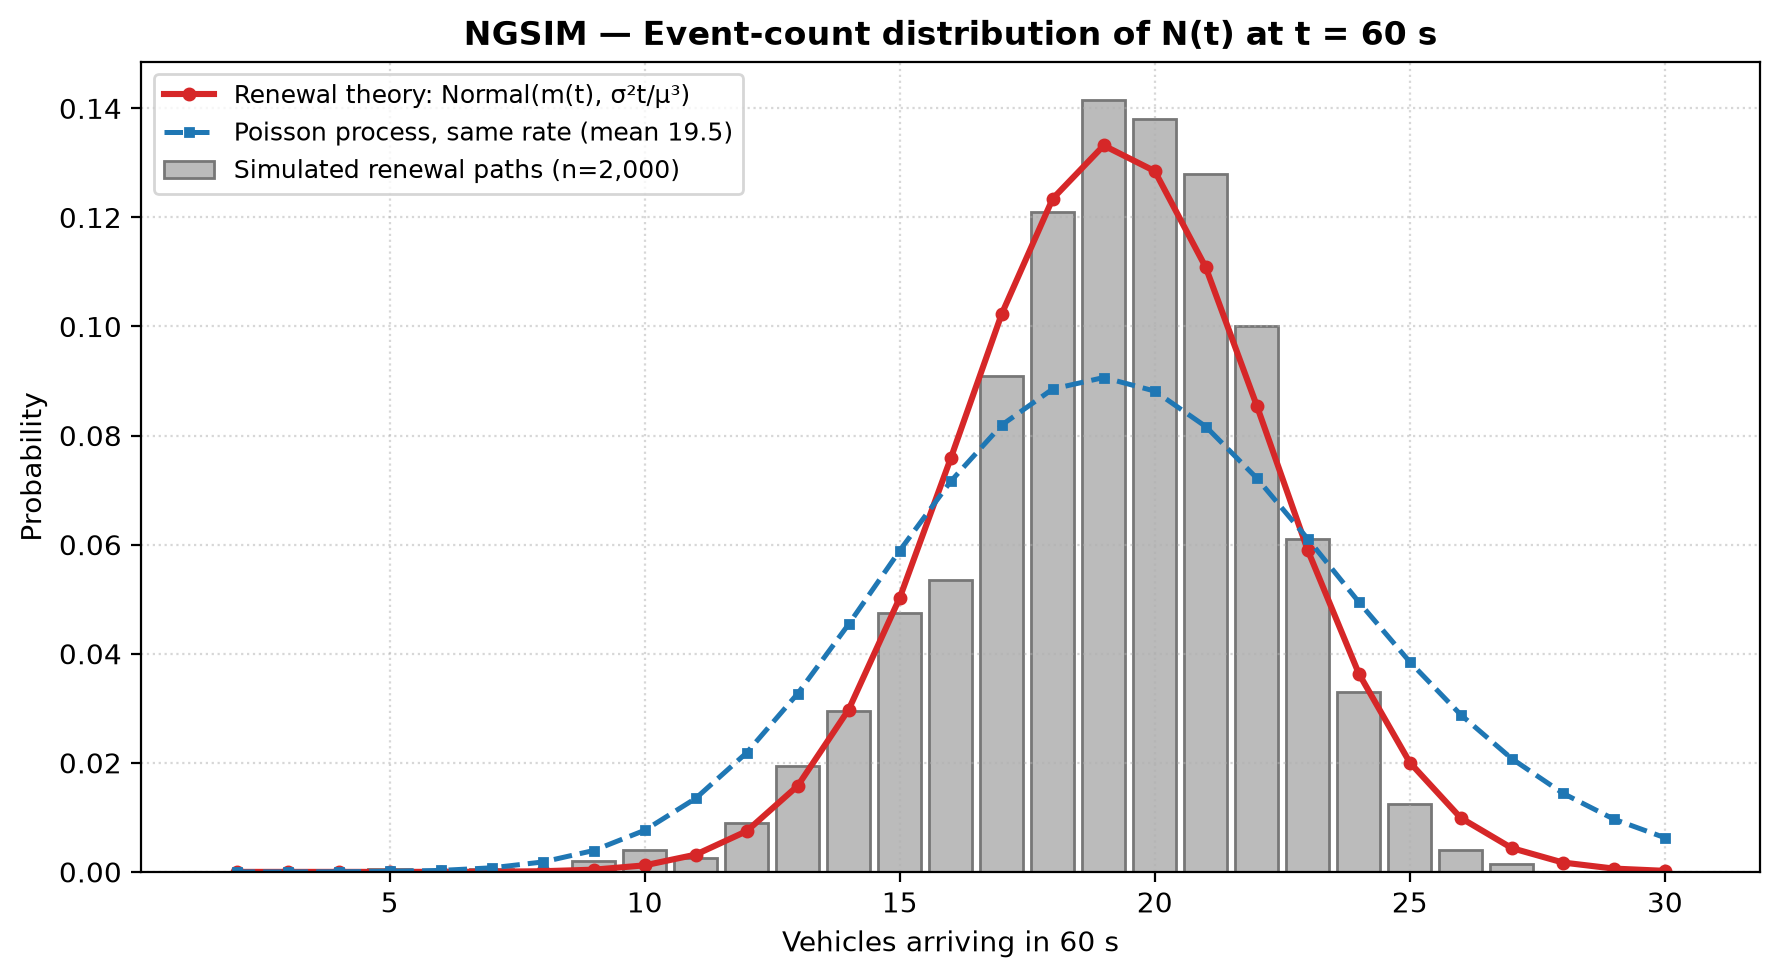
\includegraphics[width=\linewidth]{figures/ngsim_event_count.png}\caption{NGSIM}\end{subfigure}
\caption{Distribution of the arrival count $N(60\text{ s})$: simulated renewal paths (bars), the renewal-theory normal approximation (red) and a Poisson process of the same rate (blue).}\label{fig:counts}
\end{figure}

\subsubsection{Regime Markov chain}\label{sec:markovres}
Table~\ref{tab:regimes} gives the long-run behaviour of the regime chain of Section~\ref{sec:markov}. The stationary distribution coincides, to four decimals, with the observed fraction of
samples in each regime (their total-variation distance is $0.0000$ on both datasets), so the table does not depend on how the samples are ordered. The two datasets are
very different. On highD, the chain spends \hdPiC{} of the time in close following and \hdPiP{} in stable platoon, and only \hdPiF{} in free flow; on NGSIM, the platoon regime dominates
(\ngPiP), close following is rare (\ngPiC), and free flow accounts for \ngPiF. The mean recurrence times follow: a highD trajectory returns to close following on average every 2.25 steps
(seconds), whereas an NGSIM trajectory returns to it only every 10.66.

\begin{table}[htbp]
\centering\small
\caption{Stationary distribution of the regime chain (equal to the observed regime fractions) and mean recurrence times $1/\pi_i$ in one-second steps.}
\label{tab:regimes}
\begin{tabular}{@{}llrr@{}}
\toprule
Dataset & Regime & $\pi_i$ & $1/\pi_i$ (s) \\
\midrule
highD & Close following & \hdPiC & 2.25 \\
 & Stable platoon & \hdPiP & 2.32 \\
 & Free flow & \hdPiF & 7.99 \\
\midrule
NGSIM & Close following & \ngPiC & 10.66 \\
 & Stable platoon & \ngPiP & 1.38 \\
 & Free flow & \ngPiF & 5.49 \\
\bottomrule
\end{tabular}
\end{table}

The transition matrices, their state-transition diagrams, the transient evolution $\pi(n)=\pi(0)P^n$ and the Chapman--Kolmogorov checks are not reported. The runs that produced the results
of this section counted transitions between consecutive records of the loaded sample, which crosses vehicle boundaries (and, for NGSIM, was taken before the sample
was sorted by vehicle). The estimator of Section~\ref{sec:markovmethod} counts within-run transitions only; it is implemented and covered by automated tests, but its output on highD and NGSIM was not
available when this paper was prepared (Section~\ref{sec:limits}). Since $\pi$ is the marginal regime distribution, the quantities of Table~\ref{tab:regimes} are not affected.

\subsection{Real data results}\label{sec:real}
\subsubsection{Descriptive statistics}
The headway samples are summarised in Table~\ref{tab:data}. highD headways are short and concentrated (mean \hdMean~s, median \hdMedian~s); NGSIM headways are longer and more dispersed (mean \ngMean~s, median \ngMedian~s).

\subsubsection{Posterior parameter estimates}
Table~\ref{tab:params} lists the posterior means for the seven distributions next to the values published in~\cite{leungbootnak}. For the proposed distribution the highD mode is $a=\hdA$~s
(published 0.936) with $b=\hdB$ (0.540), i.e.\ a decay rate $\kappa=\hdKappa$~s$^{-1}$; on NGSIM $a=\ngA$~s (2.277), $b=\ngB$ (0.481) and $\kappa=\ngKappa$~s$^{-1}$. The highD
estimates are close to the published ones, and the NGSIM estimates are less so, which is expected from the different NGSIM sample (Section~\ref{sec:data}). The estimates of the
other distributions follow the same pattern, with the largest differences on NGSIM.

\begin{table}[htbp]
\centering\footnotesize
\caption{Posterior-mean parameters (MCMC, paper likelihood) against the published values~\cite{leungbootnak}. Parameter names are those of Table~\ref{tab:dists}.}
\label{tab:params}
\begin{tabularx}{\textwidth}{@{}lYYYY@{}}
\toprule
 & \multicolumn{2}{c}{highD} & \multicolumn{2}{c}{NGSIM} \\
\cmidrule(lr){2-3}\cmidrule(lr){4-5}
Distribution & ours & published & ours & published \\
\midrule
Proposed & $a=0.954$, $b=0.540$ & $a=0.936$, $b=0.540$ & $a=2.336$, $b=0.524$ & $a=2.277$, $b=0.481$ \\
Shifted Log-normal & $\mu=0.179$, $\sigma=0.921$, $\gamma=0.438$ & $\mu=0.233$, $\sigma=0.899$, $\gamma=0.377$ & $\mu=0.748$, $\sigma=0.614$, $\gamma=0.500$ & $\mu=0.683$, $\sigma=0.594$, $\gamma=0.528$ \\
Weibull & $\alpha=1.450$, $\beta=2.472$ & $\alpha=1.481$, $\beta=2.473$ & $\alpha=1.678$, $\beta=3.485$ & $\alpha=1.744$, $\beta=3.305$ \\
Log-logistic & $\alpha=2.618$, $\beta=1.717$ & $\alpha=2.574$, $\beta=1.719$ & $\alpha=3.664$, $\beta=2.617$ & $\alpha=3.910$, $\beta=2.515$ \\
Gamma & $\alpha=2.304$, $\beta=1.038$ & $\alpha=2.335$, $\beta=1.055$ & $\alpha=3.693$, $\beta=1.196$ & $\alpha=4.175$, $\beta=1.428$ \\
Burr & $\alpha=3.777$, $\beta=0.468$, $\lambda=1.168$ & $\alpha=3.199$, $\beta=0.602$, $\lambda=1.296$ & $\alpha=4.896$, $\beta=0.533$, $\lambda=2.086$ & $\alpha=5.237$, $\beta=0.524$, $\lambda=2.021$ \\
Shifted Exponential & $\lambda=0.584$, $\gamma=0.500$ & $\lambda=0.584$, $\gamma=0.500$ & $\lambda=0.387$, $\gamma=0.500$ & $\lambda=0.423$, $\gamma=0.558$
\\
\bottomrule
\end{tabularx}
\end{table}

\subsubsection{Goodness of fit}\label{sec:gof}
Table~\ref{tab:kl} gives the Kullback--Leibler divergence and Table~\ref{tab:wvec} the Wasserstein distance $\Wvec$ of Eq.~\eqref{eq:wvec}; Table~\ref{tab:wtime} adds the
conventional distance $\Wtime$ of Eq.~\eqref{eq:wtime} in seconds. On highD the proposed distribution has the smallest KL divergence (\hdKLprop) and the smallest $\Wvec$ (0.0012), followed by the shifted log-normal (KL 0.0063, $\Wvec$ 0.0015) and the shifted
exponential (0.0080, 0.0021); by the time-axis distance $\Wtime$ the shifted exponential is marginally ahead (0.065~s against 0.072~s for the proposed distribution). On NGSIM the Burr distribution is best by all three measures
(KL \ngKLburr, $\Wvec$ 0.0009, $\Wtime$ 0.031~s), the shifted log-normal and the log-logistic follow in KL (0.0153 and 0.0168), and the proposed distribution is fourth by all three (KL \ngKLprop, $\Wvec$ 0.0043, $\Wtime$ 0.225~s).
The ranking by KL on NGSIM, from Burr to the shifted exponential, is identical to the published ranking. On highD the published ranking differs only in that the shifted exponential and the shifted log-normal swap second and third place.
The worst fit on highD is the Weibull distribution by all three measures; on NGSIM it is the shifted exponential by KL (0.2713) and by $\Wtime$ (0.644~s) and the Weibull by $\Wvec$ (0.0090).

\begin{table}[htbp]
\centering\small
\caption{Kullback--Leibler divergence $D_{KL}$ (lower is better; best of ours in bold) against the published values.}
\label{tab:kl}
\begin{tabular}{@{}lrrrr@{}}
\toprule
 & \multicolumn{2}{c}{highD} & \multicolumn{2}{c}{NGSIM} \\
\cmidrule(lr){2-3}\cmidrule(lr){4-5}
Distribution & ours & published & ours & published \\
\midrule
Proposed & 0.0036 & \textbf{0.0036} & 0.0032 & 0.0760 & 0.0760 & 0.0805 \\
Shifted Log-normal & \textbf{0.0026} & 0.0063 & 0.0111 & 0.0153 & 0.0153 & 0.0157 \\
Weibull & 0.0079 & 0.0586 & 0.0534 & 0.1871 & 0.1944 & 0.2098 \\
Log-logistic & 0.0092 & 0.0229 & 0.0287 & 0.0167 & 0.0168 & 0.0173 \\
Gamma & 0.0075 & 0.0498 & 0.0454 & 0.1142 & 0.1150 & 0.1182 \\
Burr & 0.0043 & 0.0288 & 0.0332 & \textbf{0.0015} & \textbf{0.0016} & 0.0027 \\
Shifted Exponential & 0.0080 & 0.0080 & 0.0065 & 0.2713 & 0.2713 & 0.3024 
\\
\bottomrule
\end{tabular}
\end{table}

\begin{table}[htbp]
\centering\small
\caption{Wasserstein distance $\Wvec$ of sorted bin-probability vectors, Eq.~\eqref{eq:wvec} (unitless; lower is better; best of ours in bold) against the published values.}
\label{tab:wvec}
\begin{tabular}{@{}lrrrr@{}}
\toprule
 & \multicolumn{2}{c}{highD} & \multicolumn{2}{c}{NGSIM} \\
\cmidrule(lr){2-3}\cmidrule(lr){4-5}
Distribution & ours & published & ours & published \\
\midrule
Proposed & \textbf{0.0012} & 0.0011 & 0.0043 & 0.0040 \\
Shifted Log-normal & 0.0015 & 0.0016 & 0.0022 & 0.0021 \\
Weibull & 0.0058 & 0.0052 & 0.0090 & 0.0088 \\
Log-logistic & 0.0022 & 0.0026 & 0.0020 & 0.0020 \\
Gamma & 0.0050 & 0.0049 & 0.0063 & 0.0173 \\
Burr & 0.0033 & 0.0032 & \textbf{0.0009} & 0.0011 \\
Shifted Exponential & 0.0021 & 0.0018 & 0.0050 & 0.0047
\\
\bottomrule
\end{tabular}
\end{table}

\begin{table}[htbp]
\centering\small
\caption{Conventional one-dimensional Wasserstein distance $\Wtime$ on the time axis, Eq.~\eqref{eq:wtime}, in seconds (lower is better). The published study does not report this quantity.}
\label{tab:wtime}
\begin{tabular}{@{}lrr@{}}
\toprule
Distribution & highD & NGSIM \\
\midrule
Proposed & 0.0718 & 0.2248 \\
Shifted Log-normal & 0.1001 & 0.1544 \\
Weibull & 0.3469 & 0.5057 \\
Log-logistic & 0.1664 & 0.1649 \\
Gamma & 0.2901 & 0.3592 \\
Burr & 0.2284 & 0.0311 \\
Shifted Exponential & 0.0650 & 0.6443 \\
\bottomrule
\end{tabular}
\end{table}

Figure~\ref{fig:fits} overlays the fitted densities on the observed histograms. The statistical tests in Table~\ref{tab:tests} reject every distribution at the 5\% level on both datasets,
in the chi-square test and in the two-sample KS test, with a single exception: the chi-square $p$-value of the Burr distribution on NGSIM is $4.6\times10^{-56}$, still far below 0.05. With
samples of $10^5$ to $10^6$ observations even small departures are statistically significant, so the tests do not discriminate between the models, and the KS statistic $D$, the KL divergence and
the Wasserstein distances are more informative. The published study reports the same chi-square result (all distributions rejected) but KS $p$-values close to 1 for most distributions, whereas
ours are essentially zero; the sample sizes used for its KS test are not stated, and we do not reproduce that part of its table.

\begin{figure}[htbp]
\centering
\begin{subfigure}{0.49\textwidth}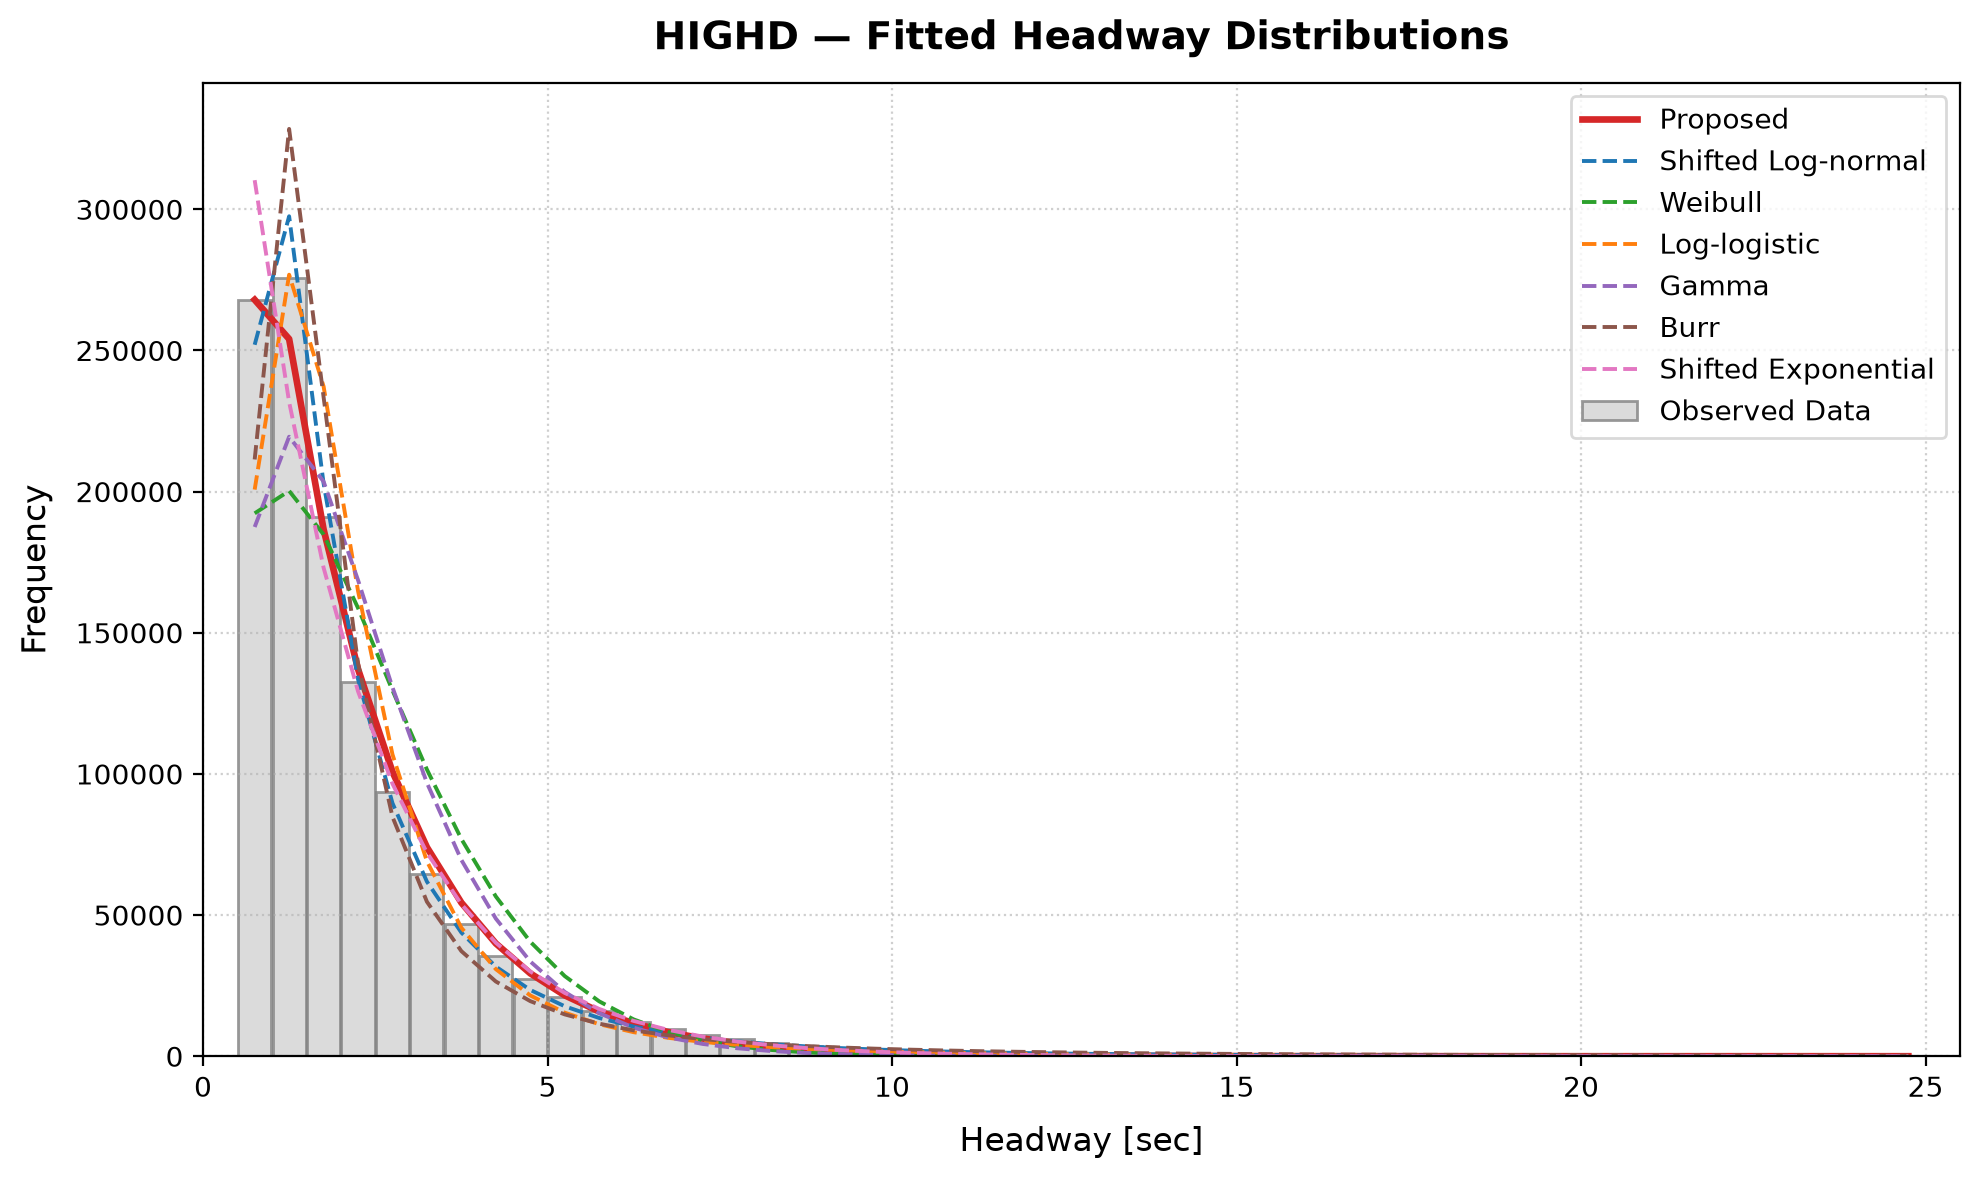
\includegraphics[width=\linewidth]{figures/highd_fitted.png}\caption{highD}\end{subfigure}\hfill
\begin{subfigure}{0.49\textwidth}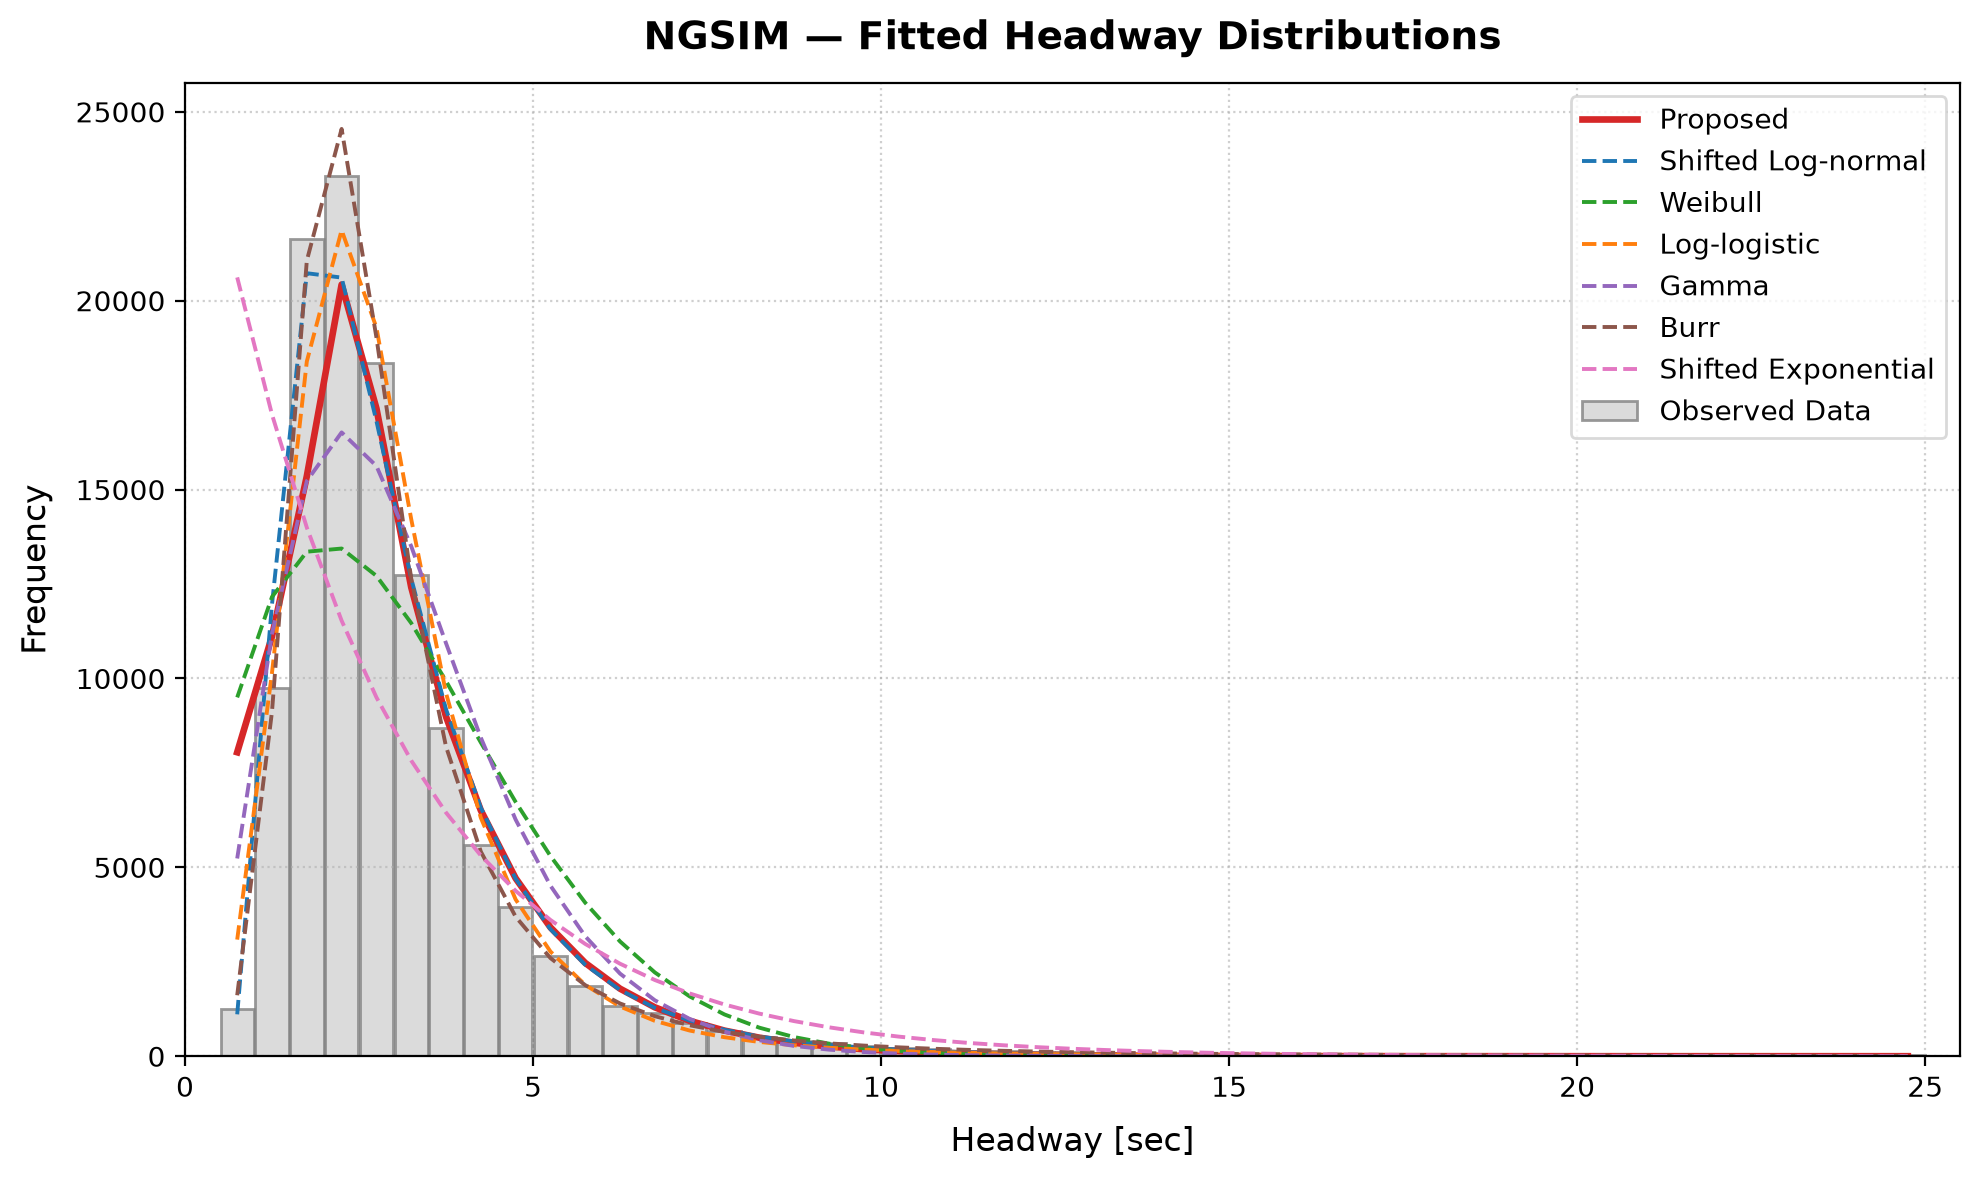
\includegraphics[width=\linewidth]{figures/ngsim_fitted.png}\caption{NGSIM}\end{subfigure}
\caption{Observed headway histogram (bars) with the seven fitted distributions; curves show the expected count per bin of the window-conditioned model.}\label{fig:fits}
\end{figure}

\begin{table}[htbp]
\centering\footnotesize
\caption{Two-sample Kolmogorov--Smirnov statistic $D$ and $p$-value, and chi-square $p$-value, for each distribution. A value below $10^{-300}$ is printed as such.}
\label{tab:tests}
\begin{tabular}{@{}lrrrrrr@{}}
\toprule
 & \multicolumn{3}{c}{highD} & \multicolumn{3}{c}{NGSIM} \\
\cmidrule(lr){2-4}\cmidrule(lr){5-7}
Distribution & KS $D$ & KS $p$ & $\chi^2$ $p$ & KS $D$ & KS $p$ & $\chi^2$ $p$ \\
\midrule
Proposed & 0.028 & $1.6\times10^{-32}$ & $<10^{-300}$ & 0.076 & $3.7\times10^{-175}$ & $<10^{-300}$ \\
Shifted Log-normal & 0.026 & $1.1\times10^{-29}$ & $<10^{-300}$ & 0.032 & $2.4\times10^{-31}$ & $<10^{-300}$ \\
Weibull & 0.137 & $<10^{-300}$ & $<10^{-300}$ & 0.128 & $<10^{-300}$ & $<10^{-300}$ \\
Log-logistic & 0.069 & $3.4\times10^{-201}$ & $<10^{-300}$ & 0.029 & $2.0\times10^{-25}$ & $<10^{-300}$ \\
Gamma & 0.118 & $<10^{-300}$ & $<10^{-300}$ & 0.095 & $5.4\times10^{-277}$ & $<10^{-300}$ \\
Burr & 0.052 & $5.2\times10^{-113}$ & $<10^{-300}$ & 0.012 & $7.0\times10^{-5}$ & $4.6\times10^{-56}$ \\
Shifted Exponential & 0.044 & $1.1\times10^{-82}$ & $<10^{-300}$ & 0.228 & $<10^{-300}$ & $<10^{-300}$
\\
\bottomrule
\end{tabular}
\end{table}

\subsubsection{highD against NGSIM}\label{sec:disc}
The proposed distribution is better suited to highD than to NGSIM, and the figure suggests why. Its density is $b^{|t-a|}$, which falls at the same rate $\kappa$ on both sides of the mode.
On highD the mode is at $\hdA$~s, only about 0.45~s above the truncation point $\alpha=0.5$~s, so that the left branch is short and the symmetric form costs little. On NGSIM the mode is at \ngA~s and the left branch
extends over about 1.8~s; the observed histogram rises much faster to the mode than it decays after it (from about 1\,200 samples in the first bin to more than 21\,000 in the third, against a decay over several seconds), and
a symmetric density with $\kappa=\ngKappa$~s$^{-1}$ overestimates the shortest headways (Figure~\ref{fig:fits}b). The three-parameter Burr, shifted log-normal and log-logistic distributions can represent this asymmetry. This explanation is read from the fitted curves and has not been tested by an
asymmetric variant of the proposed density.

\subsection{Model validation}\label{sec:valid}
Table~\ref{tab:verif} summarises what was verified, at which level (Section~\ref{sec:valstrat}), and what the result was. The subsections below give the details that
are not in earlier tables.

\begin{table}[htbp]
\centering\small
\caption{Summary of verification and validation by level.}\label{tab:verif}
\begin{tabularx}{\textwidth}{@{}lYY@{}}
\toprule
Level & Check & Result \\
\midrule
Mathematical & Closed-form CDF against numerical integration; all seven densities integrate to one; CDF derivative equals density & Pass (automated tests) \\
Simulation & MCMC recovers the known parameters of the proposed distribution from a sample drawn from it & Pass (automated test) \\
Simulation & Simulated renewal moments against Eq.~\eqref{eq:renewal} & Within \renewMeanMax\% (mean), \renewVarMax\% (variance); Table~\ref{tab:renewal} \\
Empirical & Fit of seven distributions to highD and NGSIM & Tables~\ref{tab:kl}--\ref{tab:tests} \\
Empirical & Agreement with the published results & KL within \hdKLmaxdiff{} (highD) and \ngKLmaxdiff{} (NGSIM); identical NGSIM ranking \\
Empirical & Independence of successive headways (renewal assumption) & Rejected on highD (Section~\ref{sec:indep}) \\
Empirical & Markov property and Chapman--Kolmogorov & Not reported (Section~\ref{sec:limits}) \\
\bottomrule
\end{tabularx}
\end{table}

\subsubsection{MCMC convergence}\label{sec:conv}
Table~\ref{tab:diag} gives the split $\hat R$ and acceptance rates of the real-data runs, and Figure~\ref{fig:post} and Figure~\ref{fig:trace} the posteriors and traces of the proposed distribution. For 13 of the 14 fits
the largest $\hat R$ is at most 1.011 and the acceptance rate is between 18.9\% and 26.5\%, close to the optimum of about 23\%~\cite{roberts1997}. The highD shifted-exponential fit did not converge ($\hat R=4.917$) in this run, and its estimate should not be relied upon.

\begin{table}[htbp]
\centering\small
\caption{MCMC convergence of the real-data fits: largest split $\hat R$ over the parameters (bold if $\ge1.05$) and mean acceptance rate. Two chains with 5\,000 post-warmup draws each.}
\label{tab:diag}
\begin{tabular}{@{}lrrrr@{}}
\toprule
 & \multicolumn{2}{c}{highD} & \multicolumn{2}{c}{NGSIM} \\
\cmidrule(lr){2-3}\cmidrule(lr){4-5}
Distribution & $\hat R$ & acceptance & $\hat R$ & acceptance \\
\midrule
Proposed & 1.001 & 25.6\% & 1.004 & 26.5\% \\
Shifted Log-normal & 1.003 & 21.5\% & 1.003 & 18.9\% \\
Weibull & 1.001 & 24.6\% & 1.002 & 23.2\% \\
Log-logistic & 1.002 & 23.8\% & 1.001 & 25.3\% \\
Gamma & 1.001 & 24.9\% & 1.002 & 24.0\% \\
Burr & 1.000 & 19.7\% & 1.006 & 22.9\% \\
Shifted Exponential & \textbf{4.917} & 22.5\% & 1.011 & 20.9\%
\\
\bottomrule
\end{tabular}
\end{table}

\begin{figure}[htbp]
\centering
\begin{subfigure}{0.49\textwidth}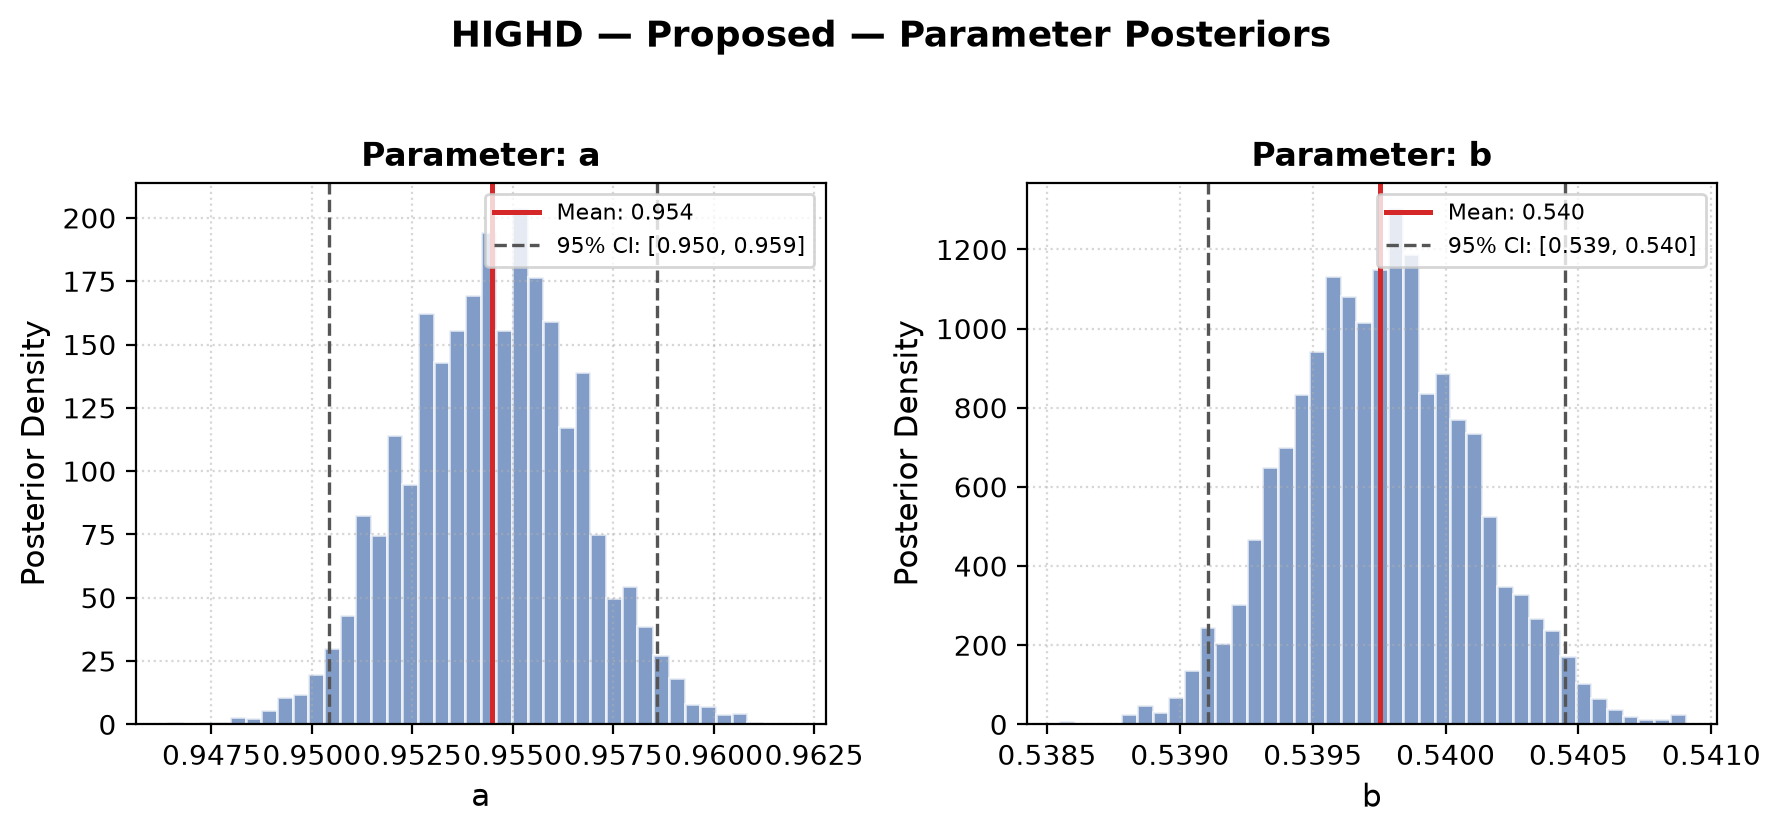
\includegraphics[width=\linewidth]{figures/highd_posterior.png}\caption{highD}\end{subfigure}\hfill
\begin{subfigure}{0.49\textwidth}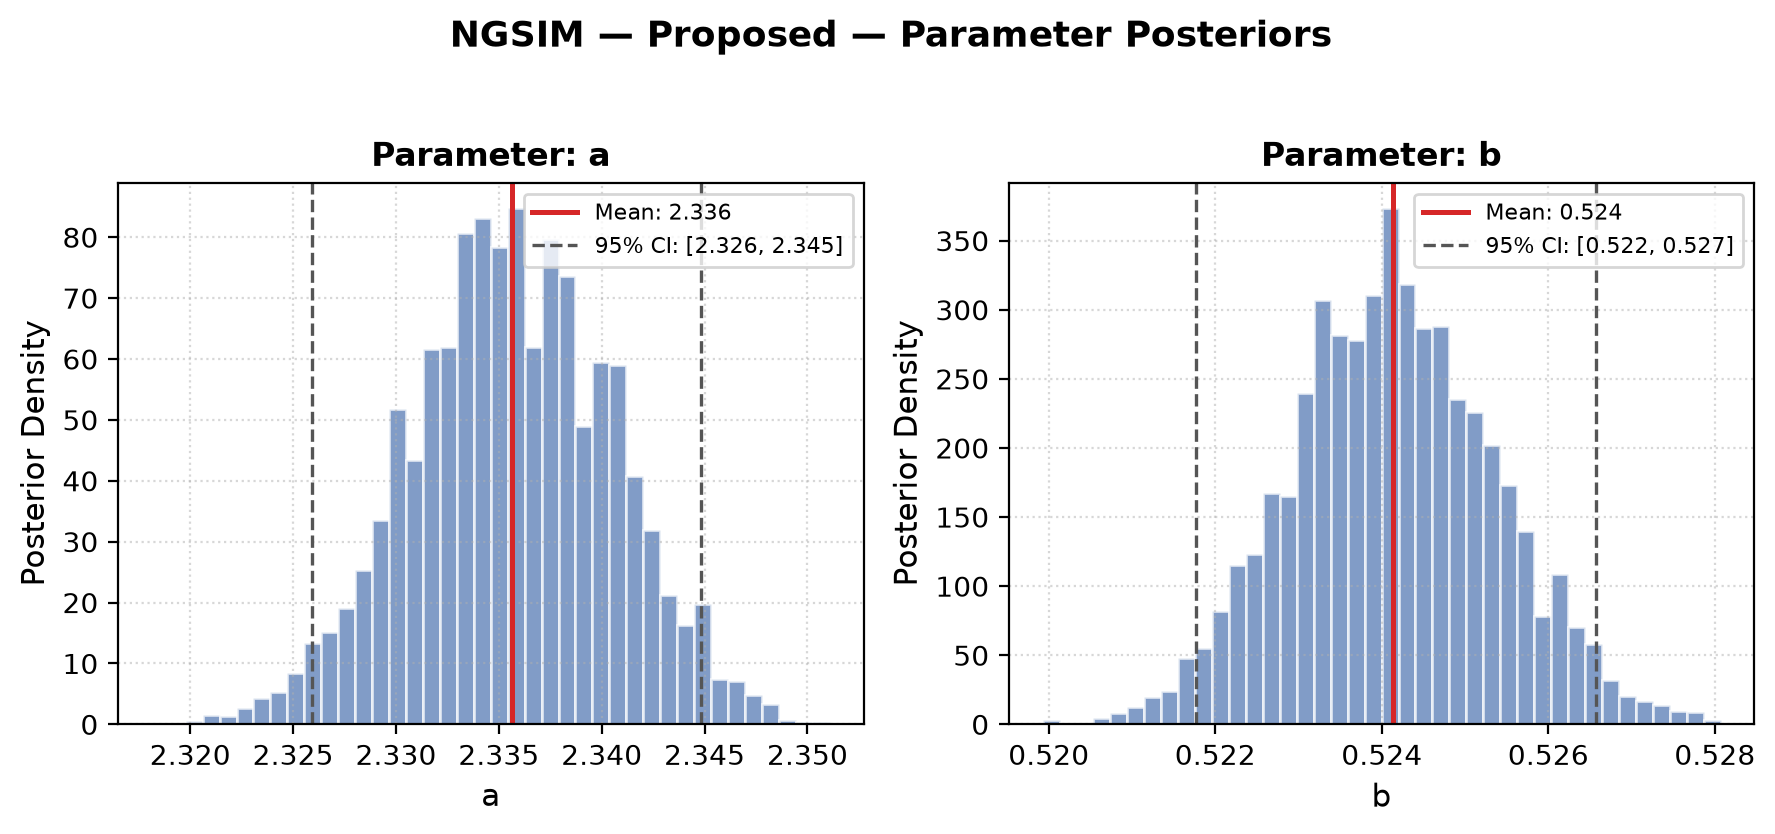
\includegraphics[width=\linewidth]{figures/ngsim_posterior.png}\caption{NGSIM}\end{subfigure}
\caption{Posterior distributions of the parameters $a$ and $b$ of the proposed distribution.}\label{fig:post}
\end{figure}

\begin{figure}[htbp]
\centering
\begin{subfigure}{0.49\textwidth}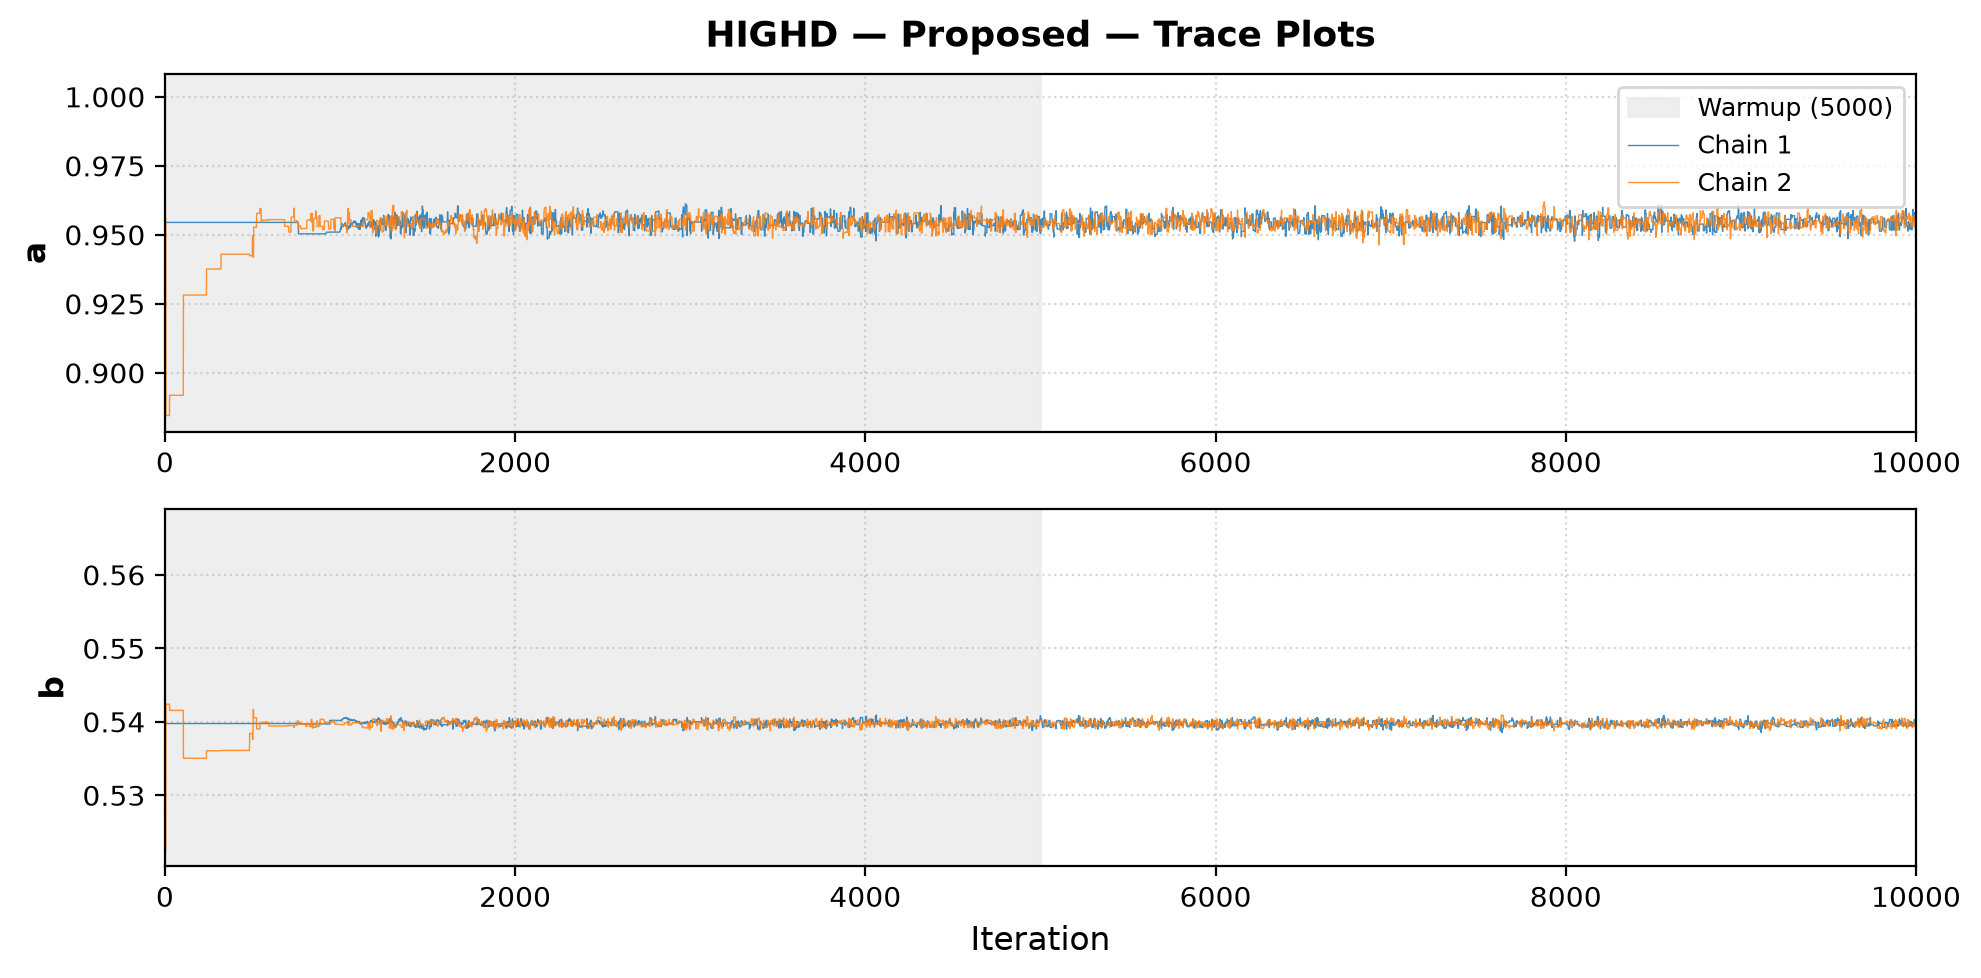
\includegraphics[width=\linewidth]{figures/highd_traces.png}\caption{highD}\end{subfigure}\hfill
\begin{subfigure}{0.49\textwidth}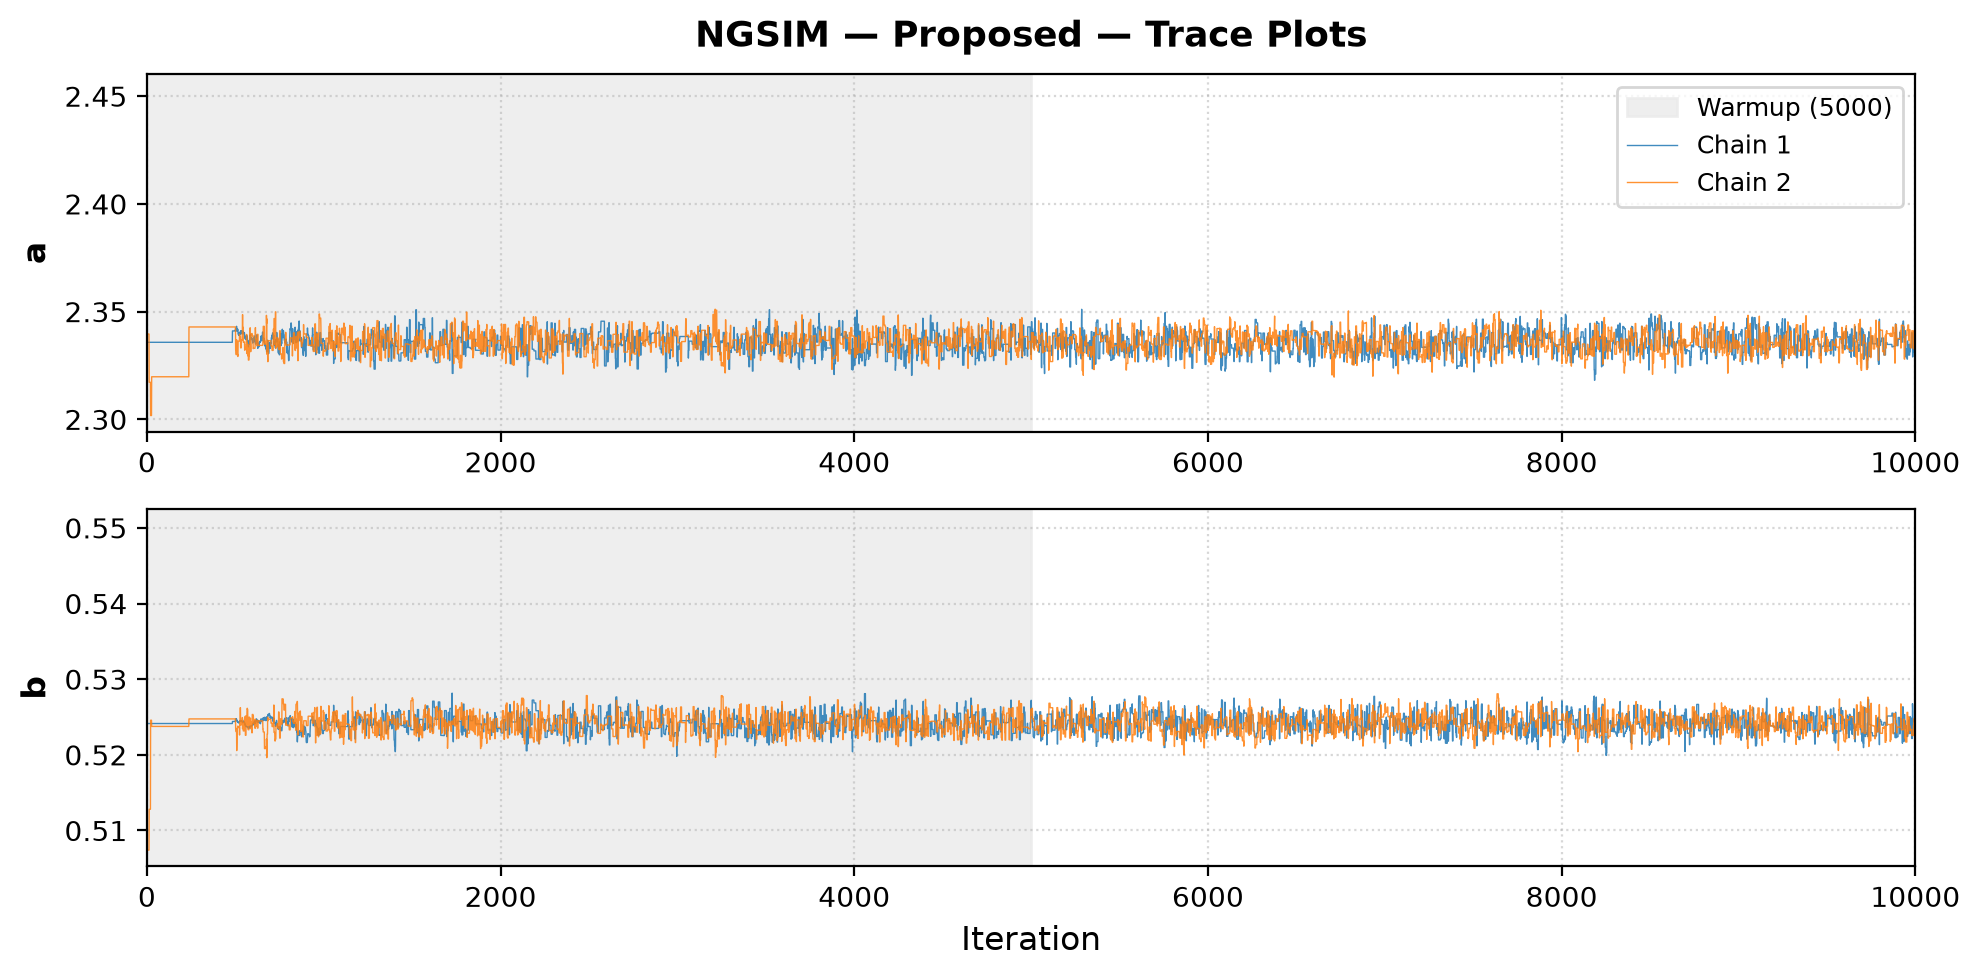
\includegraphics[width=\linewidth]{figures/ngsim_traces.png}\caption{NGSIM}\end{subfigure}
\caption{Trace plots of the two chains for the proposed distribution; the shaded part is warmup.}\label{fig:trace}
\end{figure}

\paragraph{Likely cause.} The shifted exponential has a feature that none of the other six has. For the bins above $\gamma$, the model probability of bin $k$ is
$p_k=e^{\lambda\gamma}e^{-\lambda e_k}(1-e^{-\lambda w})$ with $e_k$ the lower bin edge and $w=0.5$~s, so the binned log-likelihood contains the term $N\lambda\gamma$ and is \emph{linear} in $\gamma$, increasing without bound until $\gamma$
reaches its upper limit, the smallest observation $t_{\min}$ (the prior is $U(-10,t_{\min})$). The posterior of $\gamma$ is then close to an exponential density pressed against that limit with a scale of roughly $1/(N\lambda)$, which for $N=\hdN$ and $\lambda\approx0.58$ is of the order of $10^{-6}$~s, while
the posterior spread of $\lambda$ is of the order of $\lambda/\sqrt N\approx5\times10^{-4}$ and $\lambda$ is coupled to $\gamma$ through the same likelihood. A random walk in $(\lambda,\gamma)$ with a covariance learned during warmup is poorly matched to a ridge this thin and this close to a boundary, which is a plausible reason for chains that disagree.
This is a diagnosis from the structure of the likelihood and from the real $\hat R$ in Table~\ref{tab:diag}; it was not confirmed on the real data.

\paragraph{Correction in the code.} The sampler now works in $v=\log(t_{\min}-\gamma)$, in which the posterior is no longer pressed against a boundary, with the exact Jacobian $e^{v}$, and the MAP start is polished in the same coordinates (Section~\ref{sec:method}). A regression test with a highD-sized sample checks that $\hat R<1.05$ and that $\gamma<t_{\min}$ for every draw.
This change was made after the real-data runs reported in Table~\ref{tab:diag}; the highD shifted-exponential fit has not been repeated, so the value in the table is the one from the run before the change and is not a result of the corrected sampler.

\subsubsection{Truncation and the likelihood}\label{sec:lik}
The headways are retained only in $[0.5,25]$~s, but the published likelihood treats each distribution on its natural support: the probabilities of the 49 bins sum to less than one, which is equivalent to
assuming that the probability mass outside the window is a part of the data that happens to be unobserved. For a sample that was truncated to the window, the exact likelihood is the conditioned one, Eq.~\eqref{eq:trunc}. The two differ most when the
distribution puts appreciable mass outside the window, for example below 0.5~s or above 25~s, and not at all when it puts none there. The estimates of the baseline distributions in Table~\ref{tab:params} therefore come from a likelihood that is not exact for this sample,
while the metrics of Section~\ref{sec:gof} evaluate the fits on the conditioned distribution, so that fitting and evaluation use different distributions. This is the method of~\cite{leungbootnak}, which is what a reproduction should follow, but it means that part of the divergence of
the baseline distributions (Table~\ref{tab:kl}) may reflect the fitting method and not only the distribution family. The conditioned likelihood is implemented and selectable in the code; its effect on the real data was not measured, because the real-data runs used the paper likelihood.
Under the conditioned likelihood the shifted-exponential threshold $\gamma$ is not identifiable, because the conditioned distribution does not depend on it.

\subsubsection{Independence of successive headways}\label{sec:indep}
The renewal process of Section~\ref{sec:renewal} assumes independent headways. For highD, the autocorrelation of the sequence of retained headways at lags 1 to 5 is 0.839, 0.697, 0.575, 0.470 and 0.382
(95\% white-noise band $\pm\hdBand$), so successive one-second headways of a follower are strongly dependent and the dependence decays over several seconds. The estimate was computed in file order, where
consecutive entries of one vehicle are consecutive seconds but which also contains pairs of entries from two different vehicles, whose correlation is about zero. These pairs make it
conservative: the within-vehicle correlation is, if anything, higher than reported. The sampled one-second headways of one follower
are not the same thing as the headways between successive vehicles at a detector, which are what the renewal model describes, so the result does not show that detector inter-arrival times are dependent; it does show that the headway
sample cannot be regarded as an i.i.d.\ sample of one vehicle's behaviour, and that the renewal simulation of Section~\ref{sec:sim} models the headway \emph{distribution} and how counts accumulate under independence, not the temporal structure of the data.
For NGSIM, the equivalent computation was made before the sample was sorted by vehicle and is not reported.

\subsubsection{Markov chain}
The code for the Markov chain of Section~\ref{sec:markov} is covered by automated tests with known answers: the estimator recovers a known transition matrix, the Chapman--Kolmogorov errors are small for a true first-order chain, the
likelihood-ratio test accepts a first-order chain and rejects a second-order one, and transitions are never counted across a vehicle boundary or a gap in time. Its application to the highD and NGSIM sequences, including the
first- against second-order test, is not reported here (Section~\ref{sec:limits}).

\subsubsection{Comparison with the published results}
The KL divergences differ from the published Table~5 by at most \hdKLmaxdiff{} on highD (log-logistic) and \ngKLmaxdiff{} on NGSIM (shifted exponential), and $\Wvec$ by at most \hdWmaxdiff{} on highD (Weibull) and \ngWmaxdiff{} on NGSIM (gamma; the
other six differ by 0.0003 or less). The published $\Wvec$ for gamma on NGSIM (0.0173) is inconsistent with its own KL ranking, where gamma has a lower divergence than Weibull but twice the distance, and we do not expect any consistent
implementation to reproduce it. The remaining differences in KL are largest for the badly fitting baselines (the shifted exponential and the Weibull on NGSIM), whose divergence is sensitive to the exact sample. We could not reproduce the published sample for NGSIM,
which differs from ours in source (reconstructed against original trajectories) and probably in the selection of lanes and times. The qualitative conclusions of~\cite{leungbootnak} for these two datasets are reproduced: the proposed distribution is best on highD and the Burr distribution is best on NGSIM.

\subsection{Overall discussion and traffic interpretation}\label{sec:overall}
\paragraph{Traffic regimes.} The two datasets are in different states. The highD sample is dominated by short headways: the stationary distribution puts \hdPiC{} on close following and \hdPiP{} on stable platoon, and the lane flow
implied by the mean headway is \hdFlow{} veh/h/lane. NGSIM is dominated by platoon-range headways (\ngPiP) and its implied flow is lower (\ngFlow{} veh/h/lane). These values are the reciprocals of the mean headway of followers that have a leader, so they describe car-following states and are not flows observed at a detector.

\paragraph{Arrivals are regular, not Poisson.} The variance-to-mean ratio of the arrival count is \hdCV{} on highD and \ngCV{} on NGSIM. A Poisson model would therefore overestimate the variability of the number of vehicles in a time interval
by a factor of about 1.6 to 2.2 (the reciprocal of the ratio). This matters for applications that use arrival counts, such as queueing and signal-timing analysis, which are often built on Poisson arrivals. The regularity is what car following would be expected to
produce, since a follower adjusts its gap to the vehicle ahead and so suppresses both very short and very long headways, but the model here describes it only through the shape of the headway distribution.

\paragraph{Which distribution?} No distribution is best everywhere: the proposed distribution wins on short, concentrated highD headways and loses to more flexible, asymmetric distributions on NGSIM. This pattern, rather than the identity of
the single best model, is the practical lesson, and it is the one reported in the original study. The proposed distribution has the advantage of two interpretable parameters (the mode and the decay rate) and a closed-form distribution function that
supports exact sampling, at the cost of a symmetry constraint.

\paragraph{What the results do not show.} Because the goodness-of-fit tests reject every model, the results show relative and not absolute adequacy. The agreement of simulated renewal counts with renewal theory verifies the simulation, not the independence
assumption, which the data contradict at the one-second scale on highD.

%================================================================================================
\section{Limitations and Future Work}\label{sec:limits}

\subsection{Limitations of the present study}
\begin{enumerate}
  \item \textbf{Markov-chain results.} The transition matrices and the Markov validation of the real data (Chapman--Kolmogorov, first- against second-order) are not reported. The runs behind this paper counted transitions
        between consecutive records of the loaded sample, which crosses vehicle boundaries, and for NGSIM the records were not in vehicle-and-time order. The estimator that counts within-run transitions only, and its tests, are implemented; the
        runs of highD and NGSIM with it had not been made when this paper was prepared. The stationary distribution and recurrence times that are reported do not depend on this.
  \item \textbf{Non-converged fit.} The highD shifted-exponential fit did not converge ($\hat R=4.917$). A correction (Section~\ref{sec:conv}) is implemented but was not applied to the real data, so the estimate for that fit is not reliable.
  \item \textbf{Likelihood.} The real-data fits use the paper's likelihood, which does not condition on the truncation of the sample (Section~\ref{sec:lik}). The conditioned likelihood is implemented, but its effect on the real data was not measured. The likelihood also uses binned counts,
        exact only to the 0.5~s bin width.
  \item \textbf{NGSIM sample.} We use the original export and a recording period chosen from the published parameters, and the published sample is not reproduced. The paper does not state its sample.
  \item \textbf{Wasserstein distance.} The definition of Eq.~17 of the published study is ambiguous. $\Wvec$ matches its scale and is blind to the position of the bins; $\Wtime$ is the conventional distance. The tables report both.
  \item \textbf{Goodness-of-fit tests.} The KS $p$-values differ strongly from the published ones, whose sample sizes are not stated. All distributions are rejected by the chi-square test, as in the published study.
  \item \textbf{Renewal model.} The headways are time headways between a follower and its leader, not detector inter-arrival times, and they are not independent (Section~\ref{sec:indep}); the renewal process is a model consistent with the headway distribution.
  \item \textbf{Regimes.} The regime thresholds (1.5~s and 4~s) are modelling choices and one Markov step is one second of one vehicle.
  \item \textbf{Scope.} Two human-driven datasets, one lane at a time, no dependence on vehicle type, speed or density. The mixed human--automated datasets of the original study (Waymo, Lyft) and exiD are not included.
\end{enumerate}

\subsection{Future work}
These are proposals, not implemented work. (i)~Run the within-run Markov estimator on highD and NGSIM, and test first against second order, which would complete Section~\ref{sec:markovres}. (ii)~Repeat the real-data fits with the corrected sampler and with the truncated likelihood, and measure the change in the baselines' divergences.
(iii)~Reconstruct detector inter-arrival times from the trajectories (the time at which each vehicle crosses a fixed cross-section of a lane) and test the renewal assumption on them directly.
(iv)~Replace the first-order chain by a semi-Markov or higher-order model if the dependence between successive headways requires it. (v)~Give the proposed density different decay rates on its two sides, which the NGSIM fit suggests, and make
the headway distribution depend on speed and vehicle type. (vi)~Extend the comparison to mixed human--automated traffic.

%================================================================================================
\section{Conclusion}\label{sec:conclusion}
Headways on two highway datasets were modelled with seven fitted distributions, a renewal arrival process and a three-regime Markov chain. By Kullback--Leibler divergence the proposed distribution
$f(t\mid a,b)\propto b^{|t-a|}$ is the best of the seven on highD (\hdKLprop) and fourth on NGSIM (\ngKLprop), where the Burr distribution is best (\ngKLburr); these are the qualitative findings of the published study, and our divergences agree with
its values to within \hdKLmaxdiff{} and \ngKLmaxdiff. A symmetry of the proposed density about its mode is a plausible reason for its weaker performance on NGSIM. Arrivals simulated from the headways are markedly more regular than a Poisson stream (variance-to-mean ratios of
\hdCV{} and \ngCV), and the simulated counts agree with renewal theory, but the data show strong dependence between successive headways of a follower on highD, so that the renewal assumption is an approximation. The stationary regime distributions are
\hdPiC/\hdPiP/\hdPiF{} (close, platoon, free) on highD and \ngPiC/\ngPiP/\ngPiF{} on NGSIM.

The study also recorded two limitations of the estimation. The published likelihood does not condition on the truncation of the sample, and the posterior of the shifted exponential on highD did not converge in the run reported. A correction for the latter is implemented. Some analyses remain to be done on the real data (Section~\ref{sec:limits}): the within-trajectory Markov transition matrices and their validation, the corrected sampler, and the effect of the conditioned likelihood.

%================================================================================================
\bibliographystyle{unsrtnat}
\bibliography{references}

\clearpage
\appendix
% Generated by `python -m headway.make_code_appendix`: exact source of the functions named in each caption.
\section*{Appendix: Source Code}
\addcontentsline{toc}{section}{Appendix: Source Code}
The listings below are the exact source of the functions in the project repository (\texttt{headway/} package); they are extracted automatically, not retyped.

\lstinputlisting[caption={Density of the proposed headway distribution, normalised on $[\alpha,\infty)$ (\texttt{distributions.py}).},label={lst:pdf}]{code/proposed_pdf.py}

\lstinputlisting[caption={Distribution function of the proposed distribution, Eq.~\eqref{eq:cdf} (\texttt{distributions.py}).},label={lst:cdf}]{code/proposed_cdf.py}

\lstinputlisting[caption={Binned log-posterior used by the sampler; \texttt{likelihood} selects the paper's or the truncated likelihood (\texttt{fit.py}).},label={lst:logpost}]{code/make_logpost.py}

\lstinputlisting[caption={Adaptive random-walk Metropolis--Hastings sampler (\texttt{mcmc.py}).},label={lst:mh}]{code/metropolis.py}

\lstinputlisting[caption={One MCMC chain, including the log-gap coordinates for the shifted exponential (\texttt{fit.py}).},label={lst:chain}]{code/chain.py}

\lstinputlisting[caption={Trajectory runs: consecutive seconds of one vehicle (\texttt{datasets/common.py}).},label={lst:segments}]{code/segment_ids.py}

\lstinputlisting[caption={Markov transition estimation from within-run pairs only (\texttt{stochastic\_process.py}).},label={lst:markov}]{code/from_headways.py}

\lstinputlisting[caption={Simulation of the renewal counting process $N(t)$ (\texttt{validation.py}).},label={lst:renewal}]{code/simulate_counts.py}

\lstinputlisting[caption={Simulated moments of $N(t)$ against renewal theory (\texttt{validation.py}).},label={lst:rv}]{code/renewal_validation.py}

\lstinputlisting[caption={Chapman--Kolmogorov, stationarity and first- against second-order checks (\texttt{validation.py}).},label={lst:mv}]{code/markov_validation.py}


\end{document}
